\section{Polar Decoder}
\lecture{4 Mar.}

As was mentioned at the end of the last section, the decoding procedure to the polar code is different from that of the encoder, and one has to go backwards and forwards between layers. The following discussion focuses on multi-layered polar codes with encoding and decoding boxes of size $2\times 2$. However, the size of encoding and decoding boxes can be $2\times2$, $3\times3$, or even $\ell\times\ell$. Please refer to Fig. 2, 3, and 4 of the paper  ``Polar Codes' Simplicity, Random Codes' Durability'' \cite{Polar_Code_Simplicity} for a more general and rigorous description of the below analysis.

\begin{figure}[h]
    \centering
    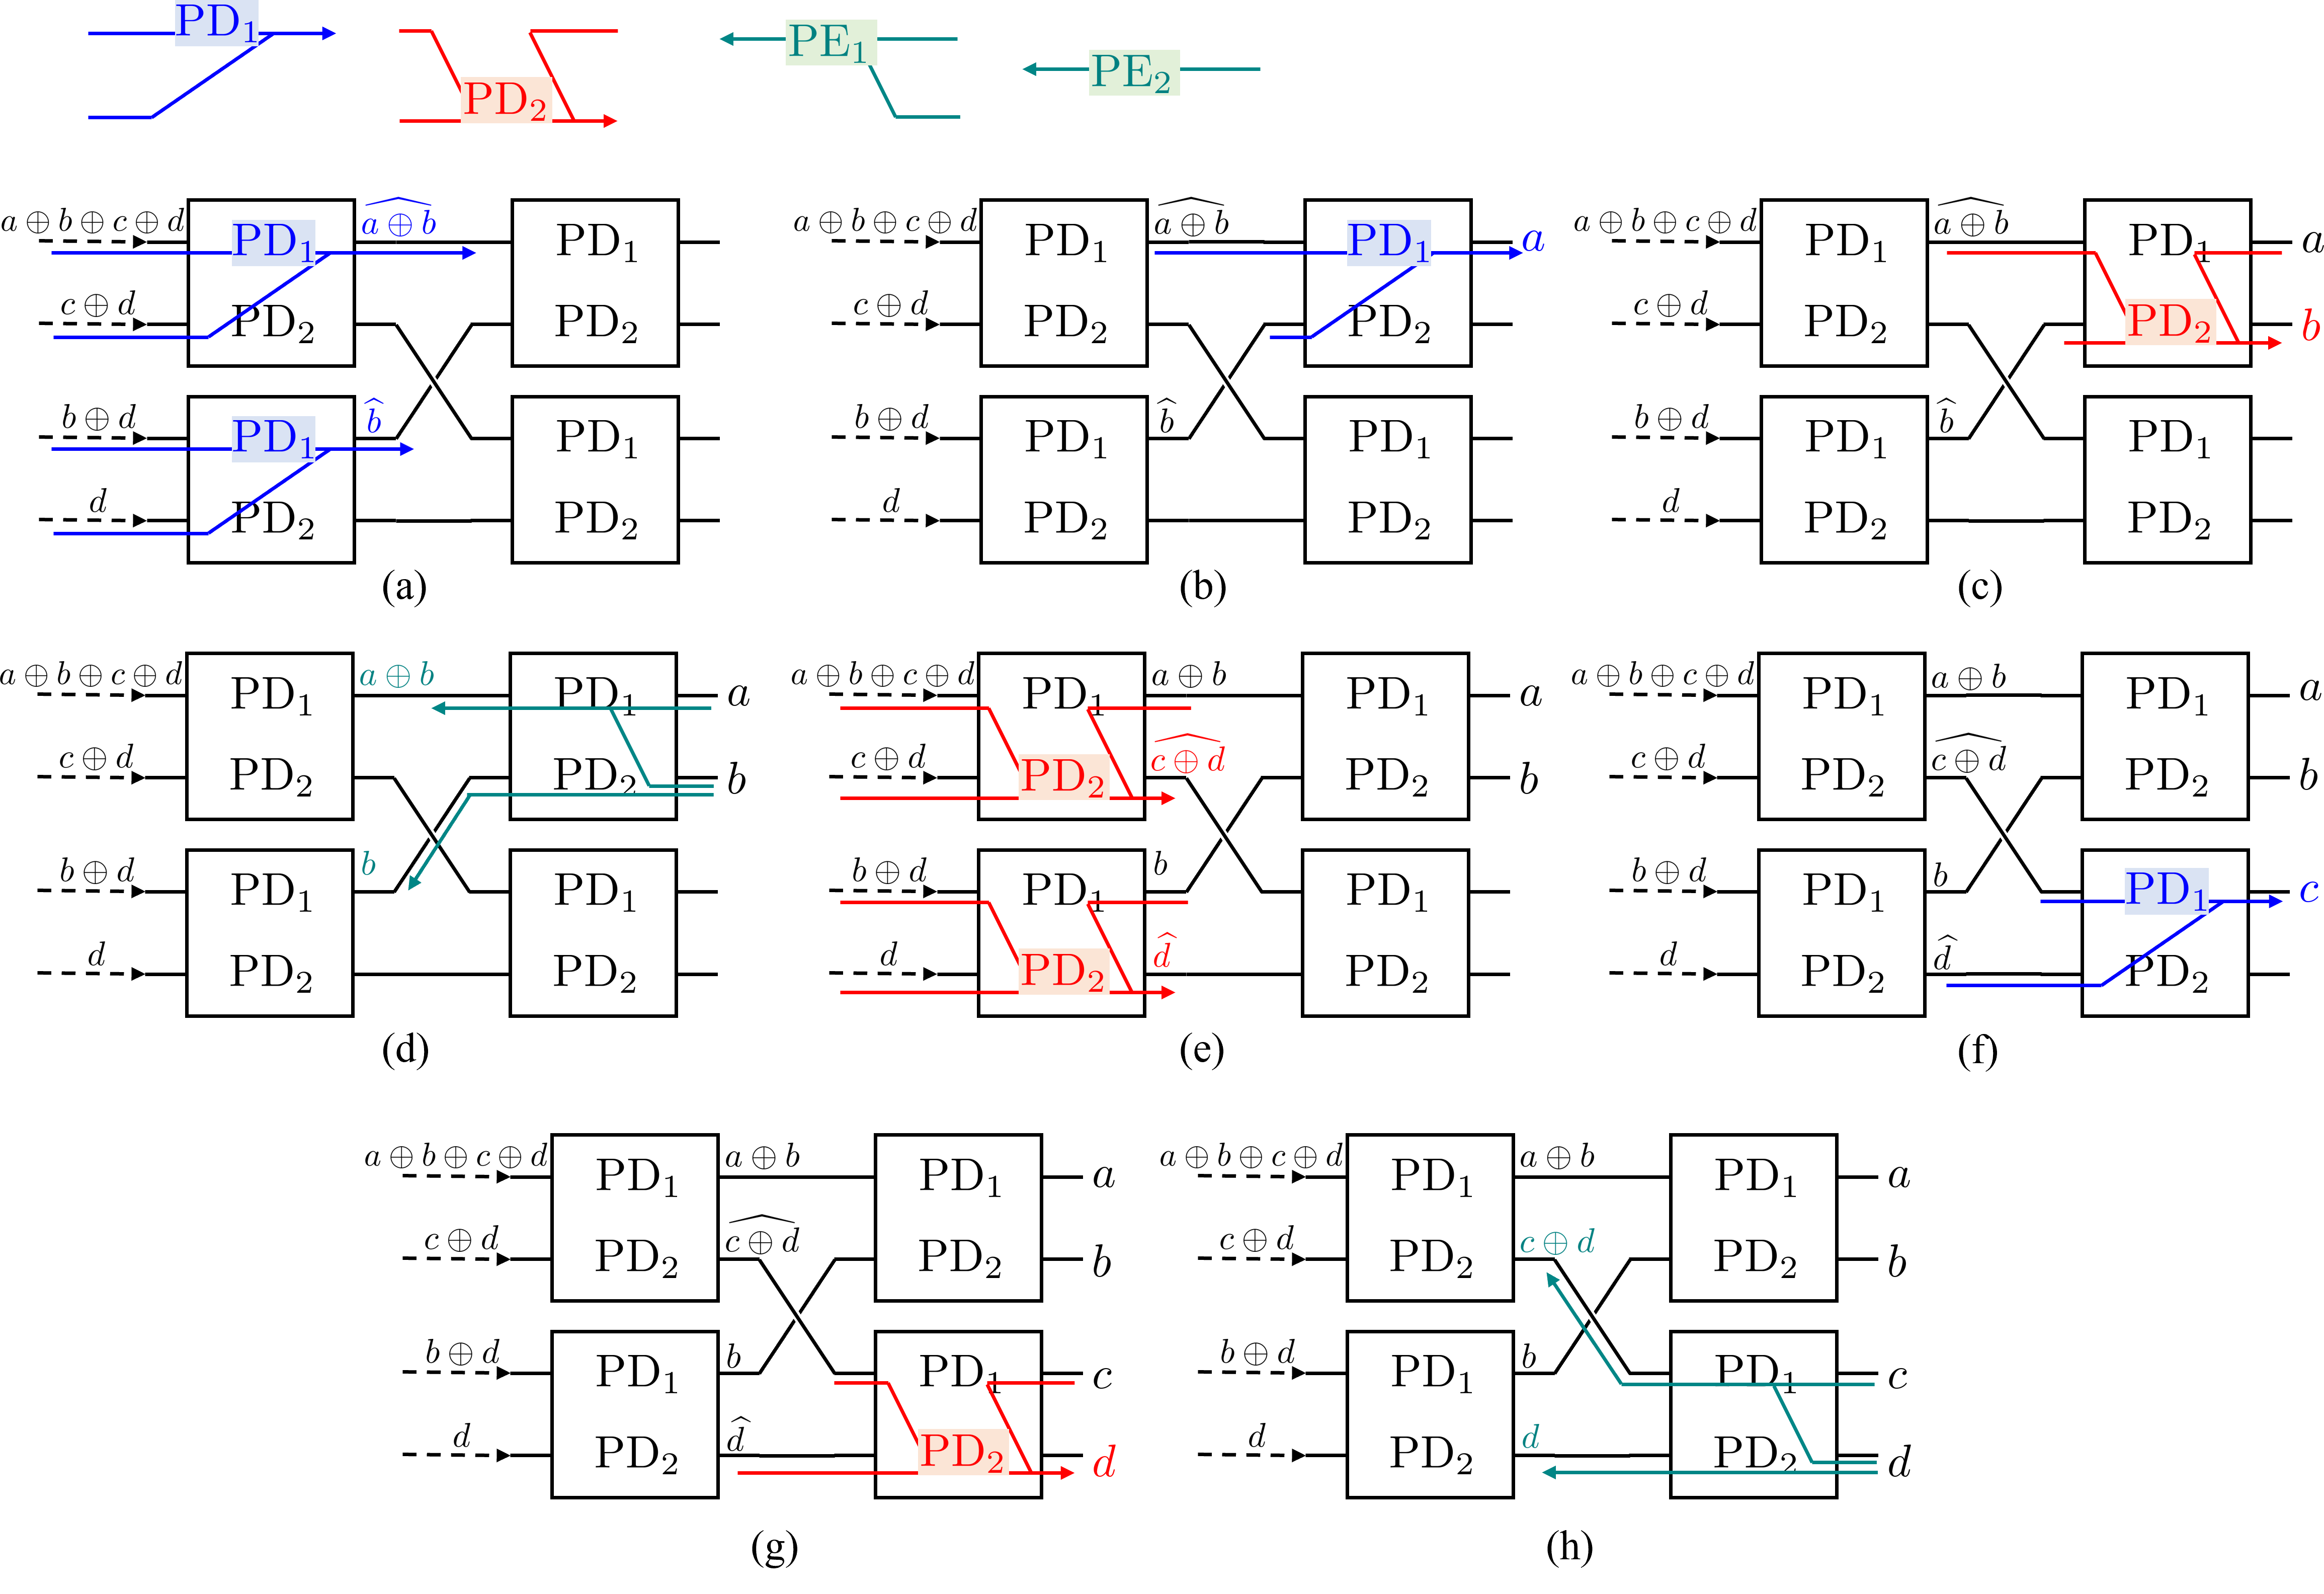
\includegraphics[width=1\linewidth]{figures/w3_2layer_decode.png}
    \caption{Decoding procedure of a two-layer polar code.}
    \label{fig:w3_polar_decoder}
\end{figure}

See the decoding procedure \autoref{fig:w3_polar_decoder} for a 2-layer polar code. Going from (a) to (h), the decoders sequentially went through the $\mathrm{PD}_1$'s and $\mathrm{PD}_2$'s. Note that since $\mathrm{PD}_2$'s require the knowledge of $u_1$'s, the box on their left will send the values by back propagating through $\mathrm{PE}_1$'s and $\mathrm{PE}_2$'s, here denoted by the teal arrows in the figure above. Moreover, we only treat the values obtained at the final column as the \textit{true} $u_1$'s.

Similar procedures can be drawn for 3-layer polar codes or more, and is left as an exercise for the readers.

The decoding of $\mathrm{PD}_2$ requires the back-propagation of true values via the polar encoders, however, what if the obtained true values are the error $\mathcal{E}$? Recall from \autoref{rmk:1.2}, it is stated that we can agree on sending $0$ over \textit{bad sub-channels} that are more erroneous. Consider having a genie\footnote{A genie is chosen since Ar{\i}kan is Turkish.} that tells us, for example, there are 4 good and 4 bad sub-channels in the 3-layer polar code as in \autoref{fig:w3_genie_aided}\footnote{What is the channel capacity implied by this distribution of good and bad channels? And no, this footnote is not an exponent.}. We can send information bits (IB) over the good sub-channels, and send frozen bits (FB) over the bad sub-channels. As mentioned, the frozen bits are chosen to be 0.

\begin{figure}[h]
    \centering
    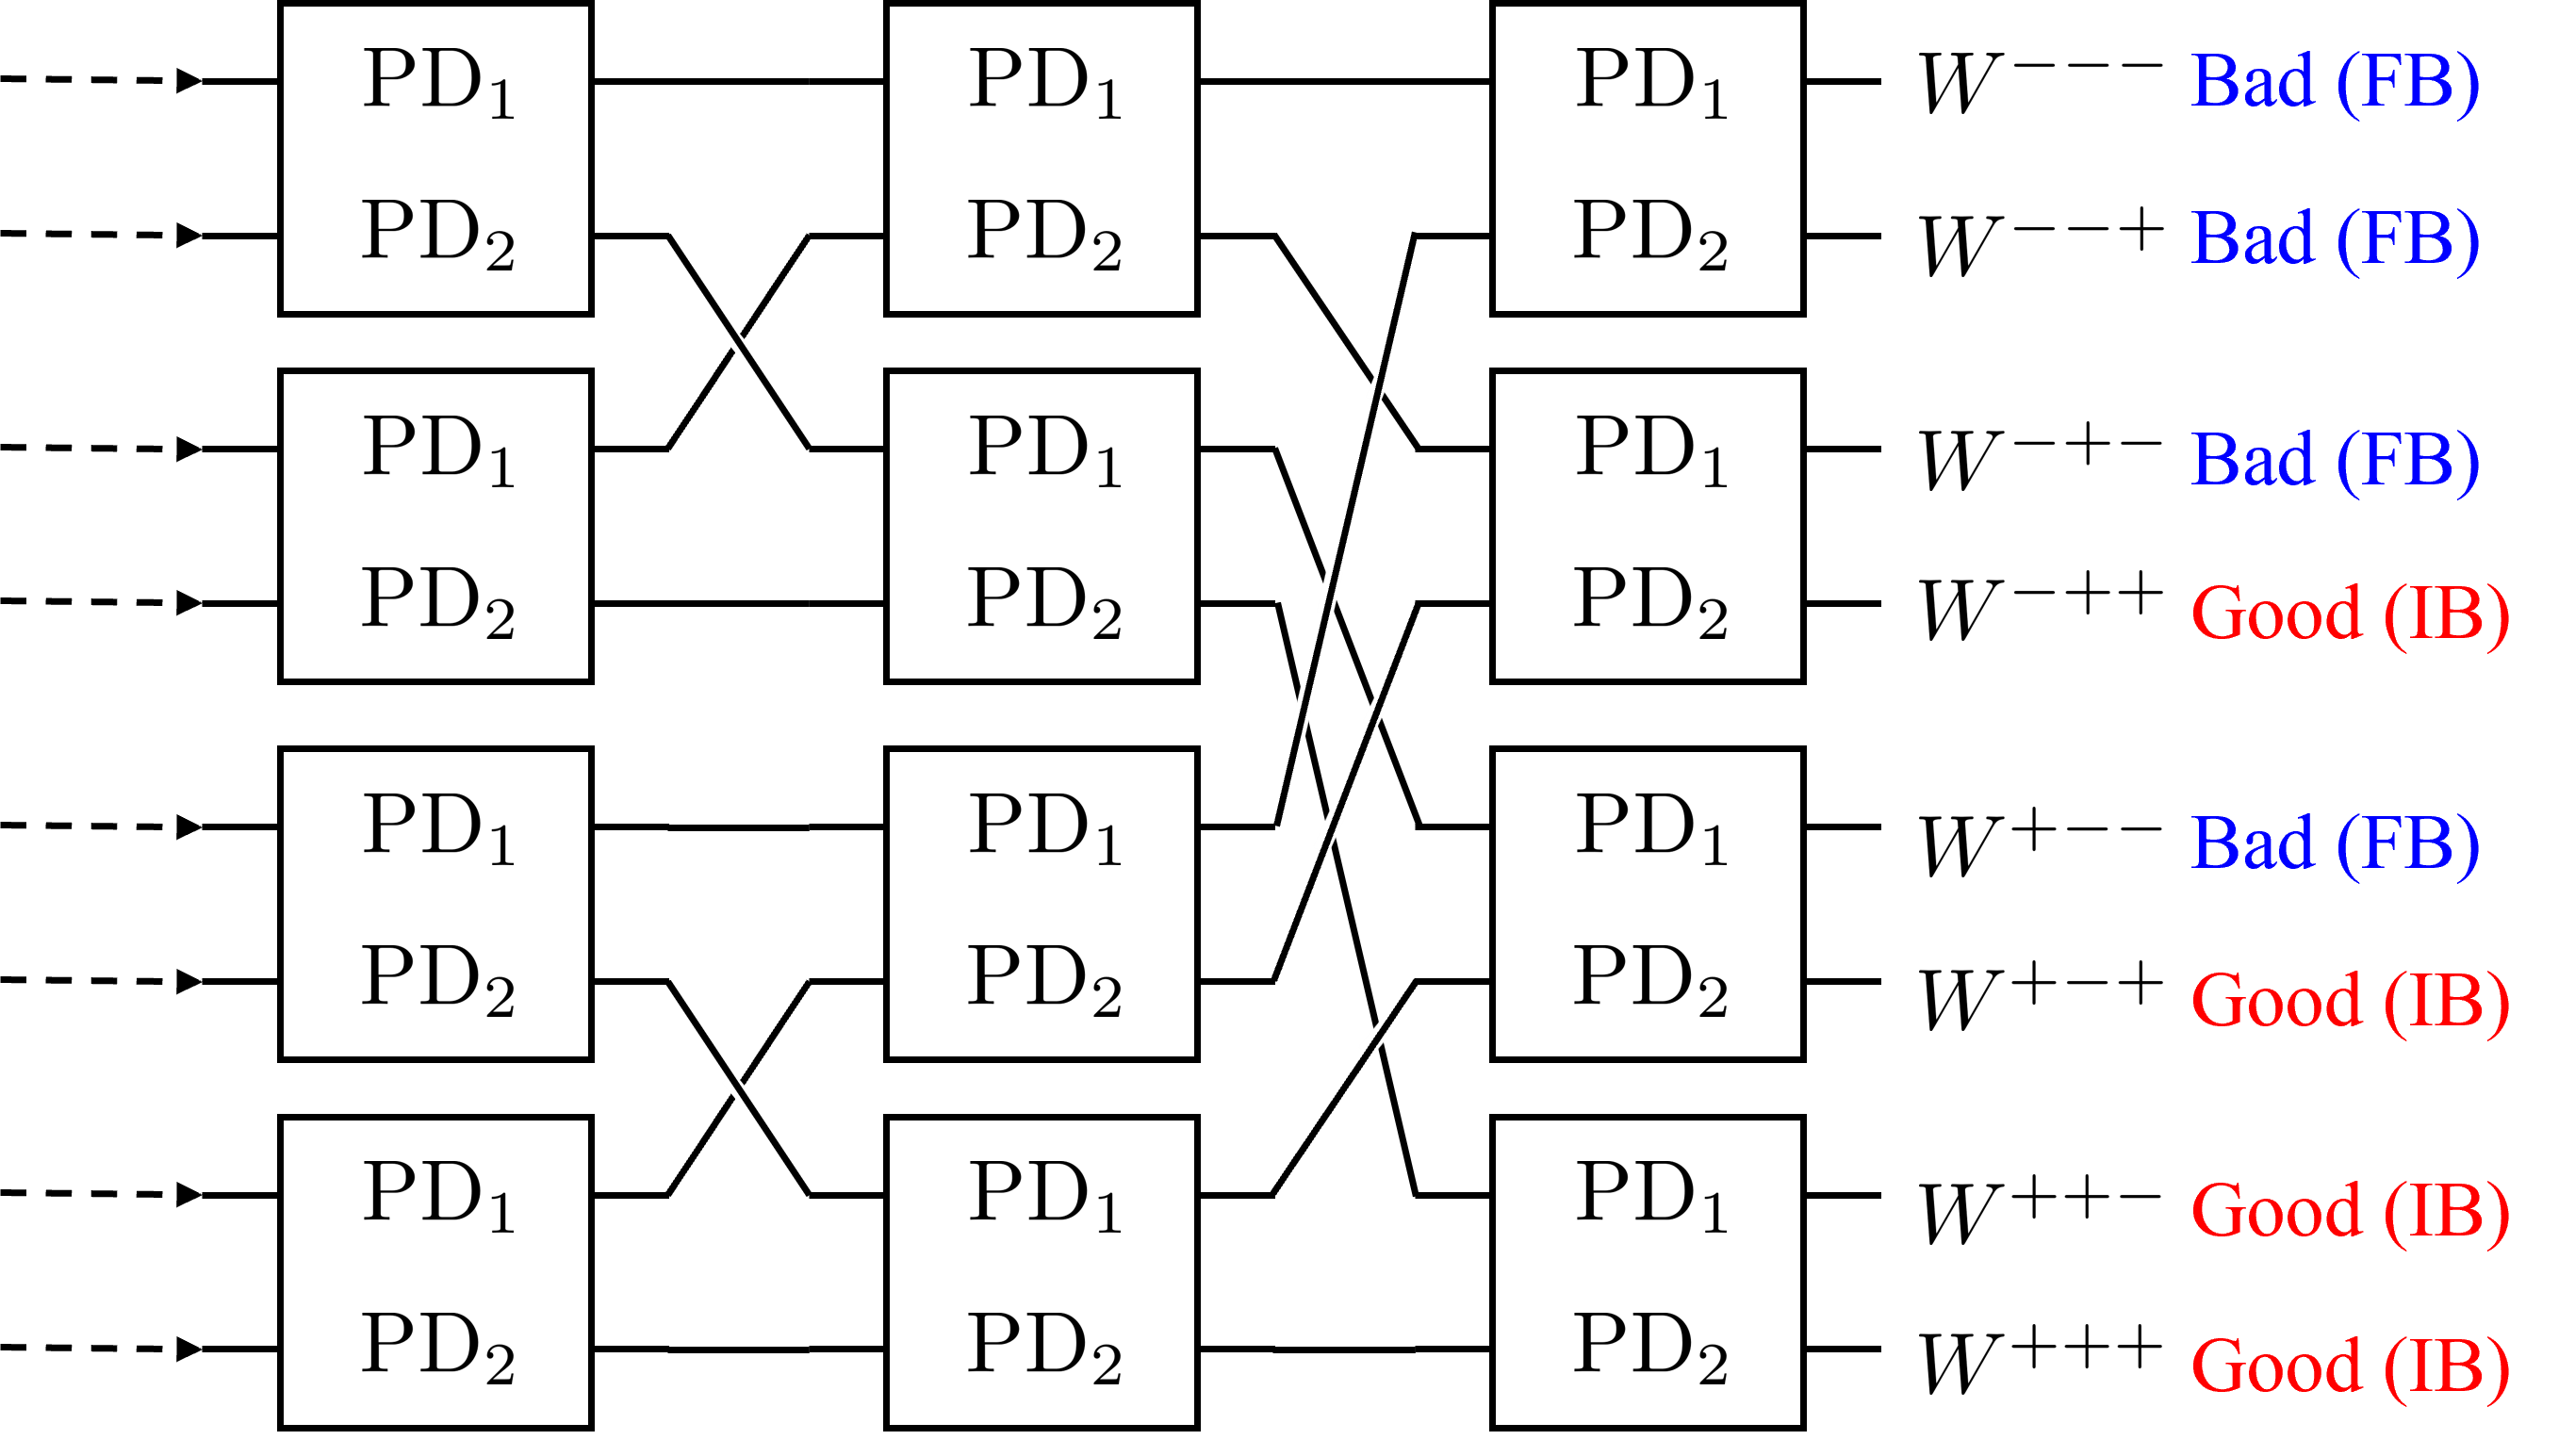
\includegraphics[width=0.6\linewidth]{figures/w3_genie.png}
    \caption{Genie-aided three-layer polar code.}
    \label{fig:w3_genie_aided}
\end{figure}

During decoding, the genie will simply send back 0 for the frozen bits as their true values; the genie will ask the decoders to figure out the true values to the information bits. One should ask themselves: why is the assignment of good and bad not \textit{continuous}? How are they determined?

Let us analyze the error probability under this scenario over BEC. Since the frozen bits can never be wrong, everything that could go wrong is when the genie gets an information bit wrong, and we simply throw out the entire block of code. The error probability will hence be: denote the polarized channels by $W^4=W^{-++}$, $W^6=W^{+-+}$, $W^7=W^{++-}$, and $W^8=W^{+++}$,
\begin{equation*}\begin{aligned}
    P_e =\; &\mathrm{Pr}\{W^{4}\text{ is wrong}\} + \mathrm{Pr}\{W^{6}\text{ is wrong}\,;\,W^{4}\text{ is right}\} \\&+ \mathrm{Pr}\{W^{7}\text{ is wrong}\,;\,W^{4},W^{6}\text{ are right}\} + \mathrm{Pr}\{W^{8}\text{ is wrong}\,;\,W^{4},W^{6},W^{7}\text{ are right}\}.
\end{aligned}\end{equation*}
If $W^4$ makes mistake, then everything else doesn't matter; if $W^4$ is correct but $W^6$ is wrong, then everything else doesn't matter; if $W^4$ and $W^6$ is correct but $W^7$ is wrong, then everything doesn't matter; if only $W^8$ is wrong, then the block is still discarded. This is also a result from the fact that the polar code is decoded sequentially. Note that from \autoref{eq:w1_bec+} and \autoref{eq:w1_bec-}, we have
\begin{equation*}
    P_e = \left((2x-x^2)^2\right)^2 + (2x^2-x^4)^2 + (2x^4-x^8) + (x^8).
\end{equation*}

The above analysis evidently shows why we choose $W^{-++}$ as a good sub-channel over $W^{+--}$.
\begin{remark}
    We choose $W^{-++}$ over $W^{+--}$ due to the fact that
    \begin{equation}
        P_e(W^{-++}) = \left((2x-x^2)^2\right)^2 \le 2(2x-x^2) - (2x-x^2)^2 = P_e(W^{+--})\;\;\;\;\;\forall\, x\in[0,1],
    \end{equation}
    with equality satisfied only at the extremals 0 and 1. See the illustration below for a clearer idea of the inequality.
    \begin{figure}[H]
        \centering
        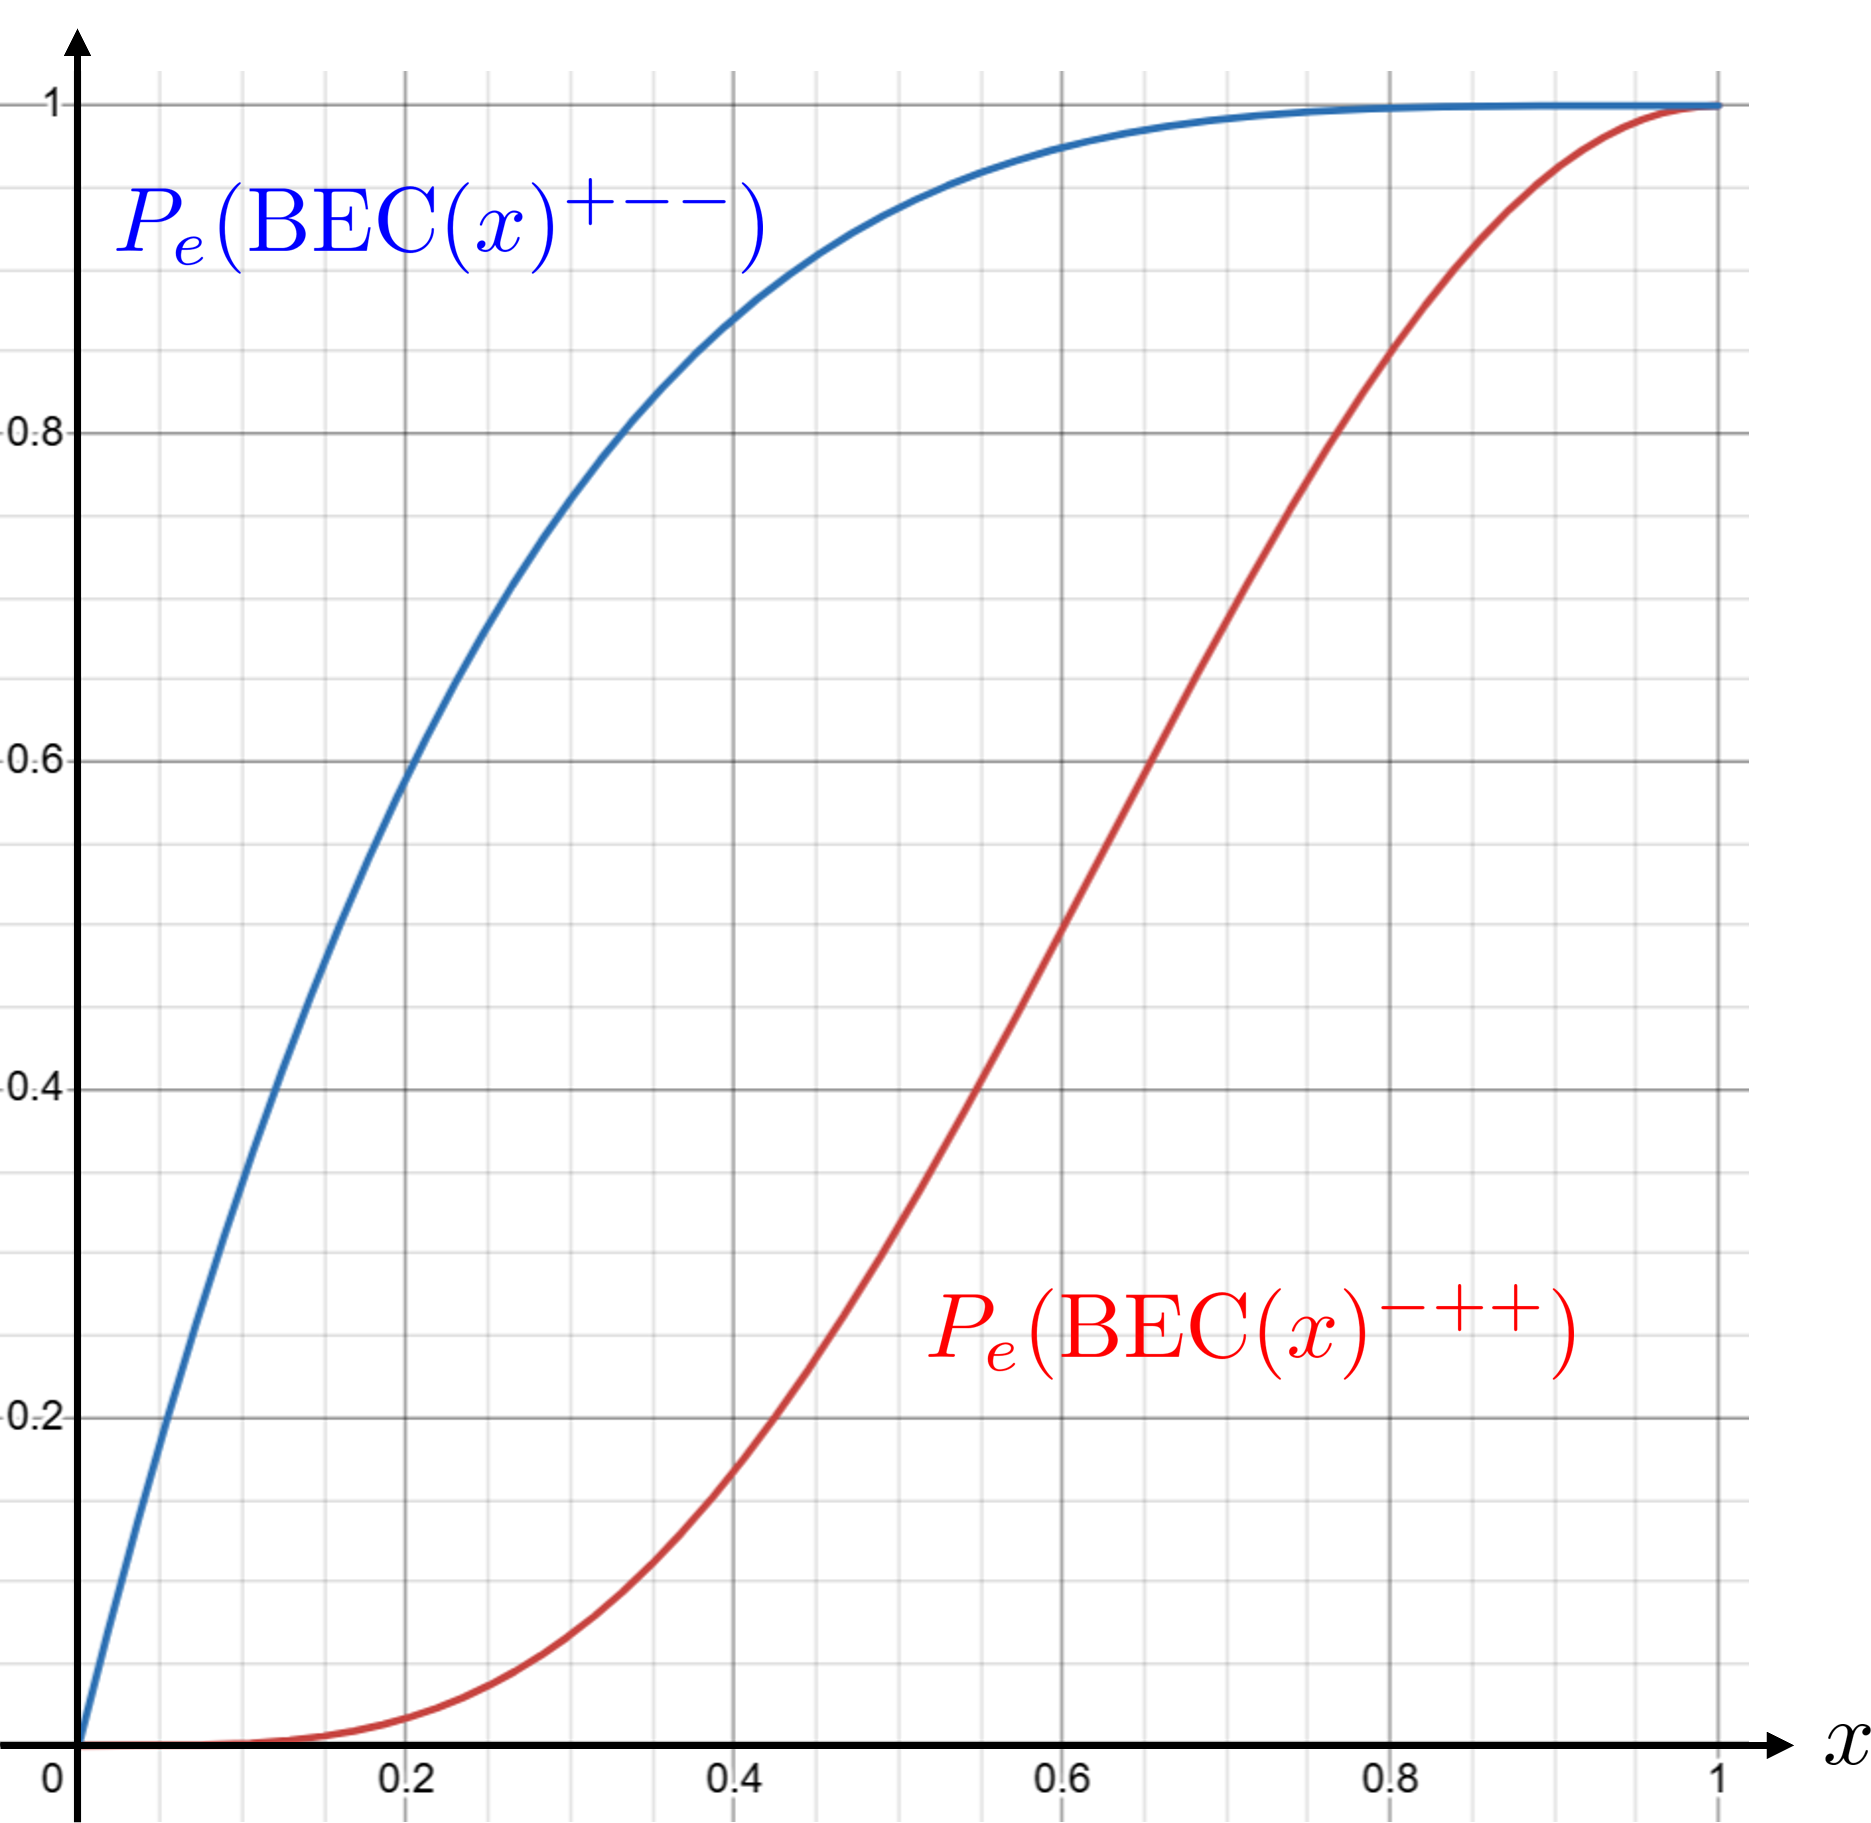
\includegraphics[width=0.35\linewidth]{figures/w3_partial_order.png}
        \caption{Ordering of the polarized error probabilities.}
    \end{figure}

    For 2-, 3-, and 4-layer polar codes over $\mathrm{BEC}(x)$, a total ordering of the sub-channels via their error probability exists.

    However, for block length greater than or equal to 32, intersections start to appear on the different error probability curves between each sub-channels. Hence, in this case, only a \textit{partial ordering} between the sub-channels exists.

    Partial-order theory is useful in deciding which sub-channel is better than which, important for the allocation of information bits, especially in the cases of long block lengths.
\end{remark}



\section{Martingale}
In this section, we take a detour and introduce the idea of a \textit{martingale}. Martingale is a special kind of random sequence that provides many useful tools from stochastic calculus in aiding our analysis of the performance of polar codes. For a proof and a more rigorous description of all the theorems below, one can refer to the book ``Probability: Theory and Examples'' \cite{Durrett} by Rick Durrett on graduate-level probability theory.

\subsection{A Brief Overview of Martingale Theory}
\begin{definition}[Martingale]
    A sequence of random variables $\{M_t\}_t$ is termed a martingale if
    \begin{align}
        &\mathbb{E}\left[\abs{M_t}\right]<\infty,&\mathbb{E}[M_{t+1}\vert M_t] = M_t.
    \end{align}
\end{definition}

Some examples of a martingale is shown below:
\begin{figure}[H]
    \centering
    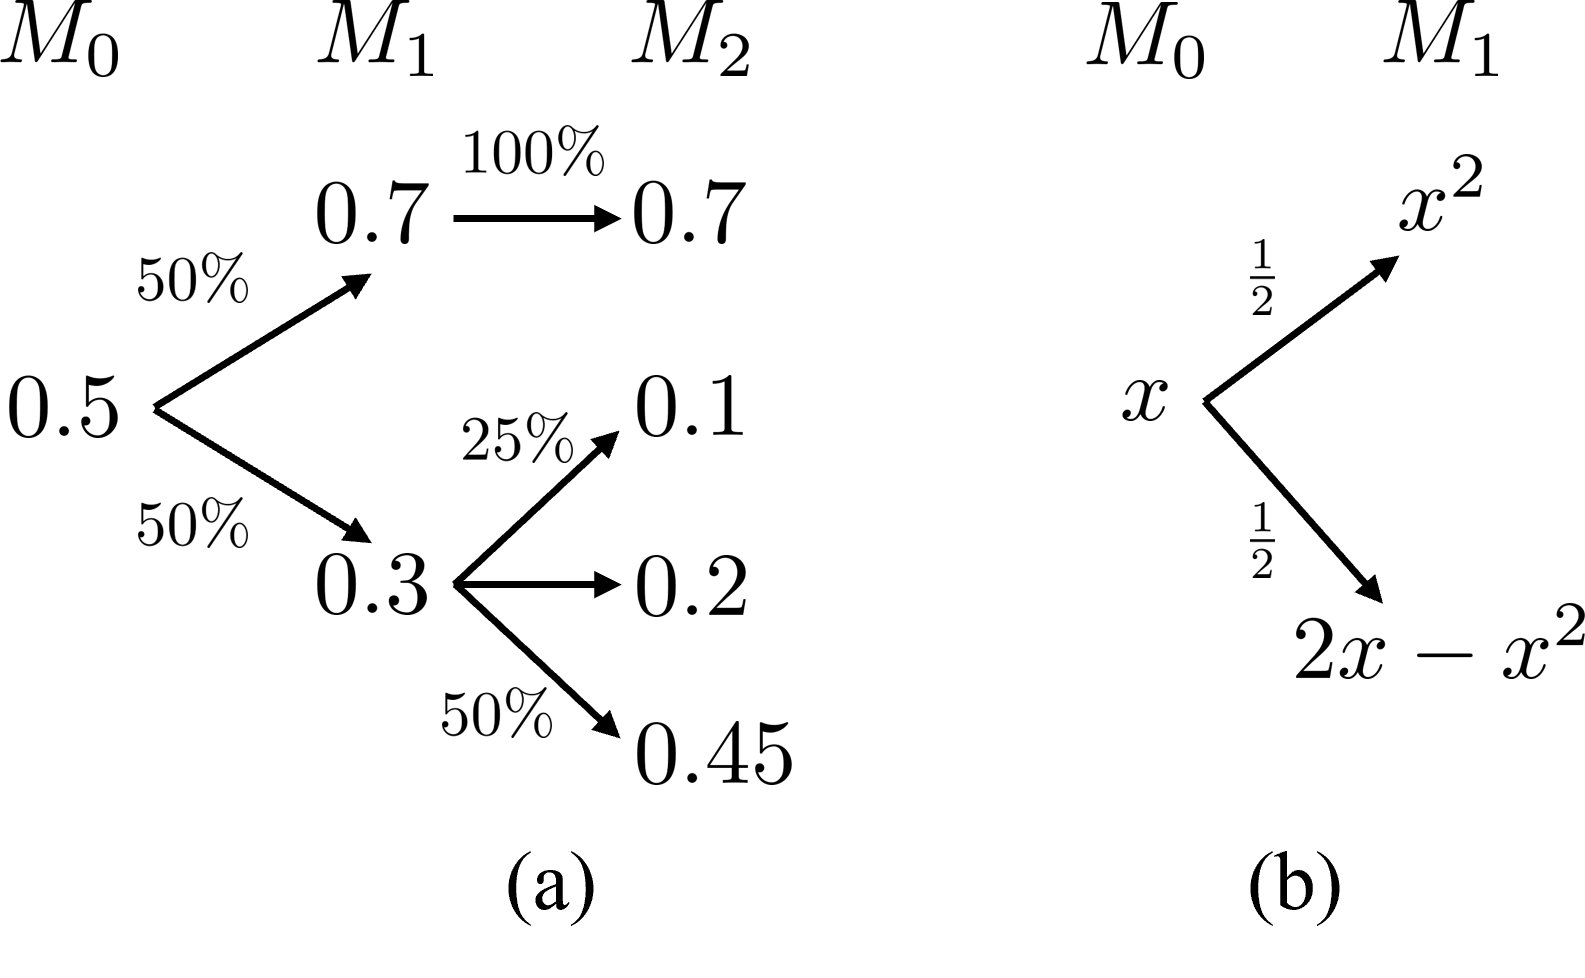
\includegraphics[width=0.5\linewidth]{figures/w3_martingale.png}
    \caption{Illustration of martingales.}
\end{figure}
One should observe that the last example given above is exactly that of the division of a BEC!

\begin{remark}
    The word ``martingale'' comes from J. Doob, the founding father of the theory of martingales. It is inspired a piece of horse gear: \textit{a long leather belt that bifurcates, at one end, into two strips of the same length}. Excerpted from ``\href{https://www.jehps.net/juin2009/Mansuy.pdf}{The origin of the word martingale},'' by Roger Mansuy.
\end{remark}

Let us now introduce the readers to a few useful theorems from the theory of martingales.
\begin{theorem}[Martingale Convergence Theorem]
    For a martingale $\{M_t\}$ that is bounded, i.e., $\abs{M_t}<\infty$\footnote{The absolutely boundedness is a really strong constraint, which can be relaxed to bounded absolute expectation.}, there exists a random variable $M_\infty$ such that $M_t\xrightarrow{\text{a.s.}} M_\infty$ as $t\rightarrow\infty$.
\end{theorem}

Here we shall give a more illustrative example showing that the theorem above is reasonable and should instinctively hold:
\begin{example}
    Define $\{M_t\}$ as the \textit{polarization process} of polar code over BEC. Let $M_0 = x$, with
    \begin{equation}
        M_{t+1} = \begin{cases}
            M_t^2 &\text{w.p. }\frac{1}{2},\\
            2M_t-M_t^2 &\text{w.p. }\frac{1}{2}.
        \end{cases}
    \end{equation}
    By the theorem above, $M_\infty$ should exist, and we further claim that $M_\infty\in\{0,1\}$.

    If $\mathrm{Pr}\left\{M_\infty=x\neq\{0,1\}\right\}\ge0$, then for all $t\ge T$, there exists a $T\gg0$ such that $M_t\in[x-\varepsilon,x+\varepsilon]$ for some fixed $\varepsilon>0$. However, $M_{T+1}$, there are 50\% chances that either of the following happens:
    \begin{align*}
        M_T^2 &\le (x+\varepsilon)^2 < x-\varepsilon,\\
        2M_T-M_T^2 &\ge 2(x-\varepsilon)-(x-\varepsilon)^2 > x+\varepsilon,
    \end{align*}
    both leading to a contradiction by choosing an $\varepsilon$ small enough. The claim that $M_\infty\in\{0,1\}$ is thus proven by contradiction.
\end{example}

\begin{example}
    Again consider $\{M_t\}$ as the polarization process of polar code over $\mathrm{BEC}(x)$. We have
    \begin{align}
        \mathrm{Pr}\{M_\infty=1\} = \mathbb{E}[M_\infty] &= \mathbb{E}\left[\lim_{t\rightarrow\infty} M_t\right] \notag\\
        &= \lim_{t\rightarrow\infty} \mathbb{E}[M_t] \label{eq:w3_martingale}\\
        &= \lim_{t\rightarrow\infty} \mathbb{E}[M_{t-1}] = \cdots = \lim_{t\rightarrow\infty} \mathbb{E}[M_0] = x. \notag
    \end{align}
    The validity of the exchange of the limit and expectation in \autoref{eq:w3_martingale} is guaranteed by the convergence of the martingale in the limit.

    Similarly, we have $\mathrm{Pr}\{M_\infty=0\} = 1-x$.
    
    Further consider a random $s\in\{+,-\}^n$, we have
    \begin{equation}\begin{aligned} \label{eq:w3_martingale_conv}
        \mathrm{Pr}\{\mathrm{BEC}(x)^s \text{ is close to }\mathrm{BEC}(1)\} &= x, \\
        \mathrm{Pr}\{\mathrm{BEC}(x)^s \text{ is close to }\mathrm{BEC}(0)\} &= 1-x.
    \end{aligned}\end{equation}
    The number of $s\in\{+,-\}^n$ such that $\mathrm{BEC}(x)^s$ is good is $2^n(1-x-\varepsilon)$, corresponding to the number of information bits; the rest of $2^n(x+\varepsilon)$ are bad, corresponding to the frozen bits.
\end{example}


\begin{definition}[Stopping Time]
    An integer random variable $\sigma$ is called a \textit{stopping time} if whether or not $\sigma\le t$ depends only on $M_1,\ldots,M_t$, and not on $M_{t+1},M_{t+1},\ldots$.
\end{definition}
\begin{theorem}[Optional Stopping Time]
    For a martingale $\{M_t\}$ with stopping time $\sigma$, we have
    \begin{equation}
        \mathbb{E}[M_\sigma] = \mathbb{E}[M_0].
    \end{equation}
\end{theorem}
The proof can be directly seen from the example above.

\begin{example}
    Let us consider a martingale $\{M_t\}$ with $M_t\ge0$. Let $M_0=0.001$ be deterministic. Define its stopping time as $\sigma\defeq\min\setdef{t}{M_t\ge1}\cup\{N\}$ where $N$ is very large. In the context of a stock market, this definition of stopping time corresponds to ones strategy of selling out when reaching a gain of profit larger than 1 with a small initial investment. Let us bound the success probability of such strategy.
    \begin{align*}
        M_0 \equiv \mathbb{E}[M_\sigma] &= \mathbb{E}\left[M_\sigma\cdot\mathbbm{1}\{M_\sigma\ge1\}\right] + \mathbb{E}\left[M_N\cdot\mathbbm{1}\{M_\sigma\text{ is never larger than }1\}\right] \\
        &\ge \mathbb{E}\left[M_\sigma\cdot\mathbbm{1}\{M_\sigma\ge1\}\right] \\
        &\ge \mathrm{Pr}\{M_\sigma\ge1\}.
    \end{align*}
    Henceforth, we have $\mathrm{Pr}\{M_\sigma\ge1\}\le M_0=0.1\%$. The probability of gaining huge profit from small investment in this model is small.
\end{example}
This result above can be generalized via the Markov inequality: given a martingale $M_t\ge0$, we have $\mathrm{Pr}\{M_\sigma\ge a\} \le \mathbb{E}[M_\sigma]/a = \mathbb{E}[M_0]/a$. This is known as Doobs's maximum inequality.
\begin{theorem}[Doob's Maximum Inequality]
    Let the optional stopping time for a martingale $\{M_t\}$ be
    \begin{equation}
        \sigma:\text{ minimum }t\text{ that }M_t\text{ reaches }A.
    \end{equation}
    Then since
    \begin{equation}
        M_\sigma \ge A \Leftrightarrow \max_t M_t \ge A,
    \end{equation}
    we have
    \begin{equation}
        \mathrm{Pr}\{\max_t M_t\ge A\} = \mathrm{Pr}\{M_\sigma\ge A\} \le \frac{M_0}{A}.
    \end{equation}
\end{theorem}
\begin{remark}
    Doob single-handedly translated the theory of martingale from a competing theory of description of probability to the now widely-used measure-theoretical probability theory.
\end{remark}
\begin{remark}
    The applications to martingale often includes stochastic calculus and stock market analysis. The concept of stopping time can be, as an example, interpreted as the time one sells out their stocks.

    Moreover, two other kinds of martingales exist:
    \begin{enumerate}
        \item Supermartingale: $\mathbb{E}[M_{t+1}\vert M_t] \le M_t$;
        \item Submartingale: $\mathbb{E}[M_{t+1}\vert M_t] \ge M_t$.
    \end{enumerate}
\end{remark}

We can proof the (Doob's) martingale convergence theorem from the Doob's maximum inequality:
\begin{proof}
    Assume that we are considering a bounded martingale $0\le M_t\le 1$. We claim that if $M_t$ does not converge, then there exists $0< a<b<1$ such that $M_t$ oscillates infinitely many times between $a$ and $b$. See the figure below:
    \begin{figure}[H]
        \centering
        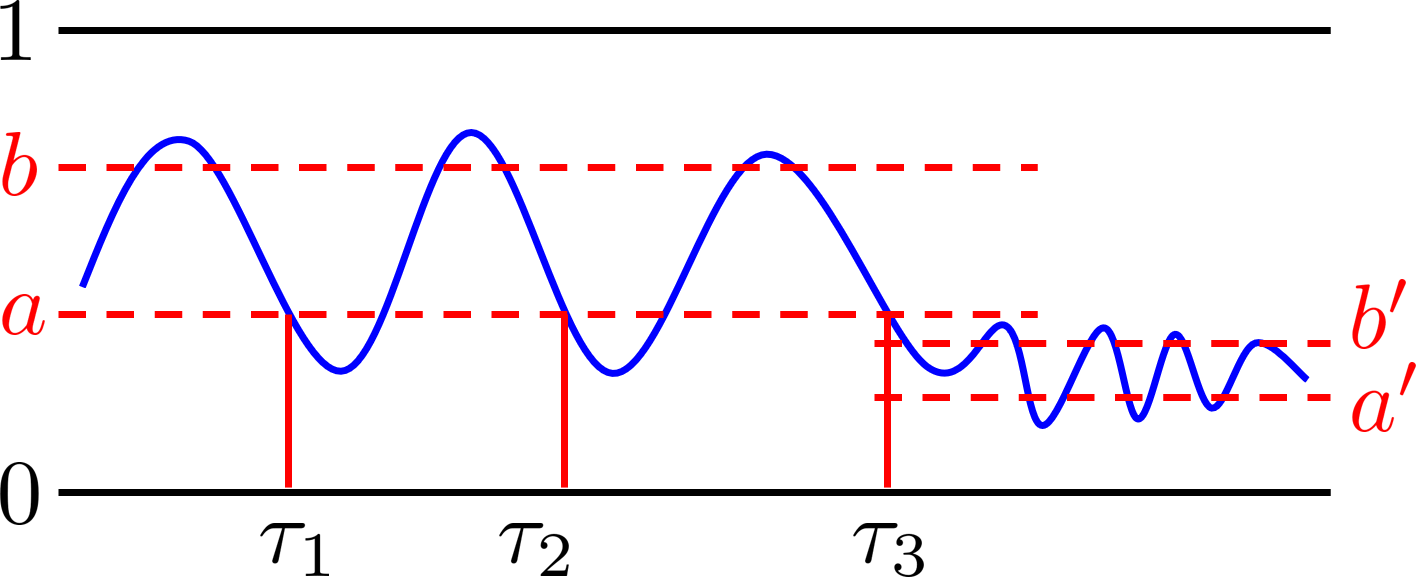
\includegraphics[width=0.5\linewidth]{figures/w4_martingale_oscillate.png}
        \caption{Illustration of the martingale convergence theorem.}
    \end{figure}
    If the martingale oscillates outside $[a,b]$, one can find another interval $[a',b']$ in which the martingale will finally reside in. Denote the time when $M_t=a$ as $\tau$'s, we have, from the maximum inequality:
    \begin{equation}
        \mathrm{Pr}\{M_{\tau+t}\ge b\vert M_\tau=a\} \le \frac{a}{b} <1.
    \end{equation}
    Since the oscillation happens infinitely many times, we have the total probability $(\frac{a}{b})^n\rightarrow 0$. Thus, if the sequence doesn't bound between 2 numbers, it must be \textit{almost surely} convergent.
\end{proof}

\subsection{McDiarmid's Inequality}
Recall from large deviation theory that we have, for i.i.d. and bounded random variables $X_1$, $\ldots$, $X_n$,
\begin{equation}
    \mathrm{Pr}\left\{\frac{X_1+\cdots+X_n}{n} - \mathbb{E}[X_1] \ge \varepsilon\right\} \le \exp(-c\varepsilon^2n)
\end{equation}
for some constant $c$. This is known as the Chernoff bound or Hoeffding's inequality.

A similar version for martingale exists:
\begin{theorem}[Azuma's Inequality]
    For a martingale $\{M_t\}$ with bounded variation $\abs{M_{t+1}-M_t}\le C$, we have
    \begin{equation}
        \mathrm{Pr}\left\{\frac{M_n}{n}-M_0 > \varepsilon\right\} < \exp(-c\varepsilon^2n)
    \end{equation}
    for some constant $c$.
\end{theorem}
This inequality can be used to show the capacity-achieving property of polar codes. Moreover, by defining $M_t$ as
\begin{equation}
    M_t \defeq X_1+\cdots+X_t - t\cdot\mathbb{E}[X_1],
\end{equation}
we can see that it is indeed a martingale:
\begin{equation*}
    \mathbb{E}[M_{t+1}\vert M_t] = M_t + \mathbb{E}\left[X_{t+1}-\mathbb{E}[X_1]\right] = M_t.
\end{equation*}
We readily obtained the Hoeffding's inequality from Azuma's inequality.

This result can, obviously, be further generalized. Let us define some similar notions needed for the description of the following theorem.
\begin{definition}[Bounded Variation]
    A function $f:[0,1]^n\rightarrow \mathbb{R}$ is of bounded variation if there exists a $C_i$ such that
    \begin{equation}
        \abs{f(a_{1:i-1},b_i,a_{i+1:n}) - f(a_{1:i-1},c_i,a_{i+1:n})} < C_i
    \end{equation}
    is satisfied for all possible $i$, $b_i$, and $c_i$.
\end{definition}
\begin{definition}[Doob's Martingale]
    For an $n$-variable function $f$, the following sequence is a martingale:
    \begin{align}
        M_0 &= \mathbb{E}_Y[f(Y_{1:n})], \\
        M_t &= \mathbb{E}_{Y_{t+1:n}}[f(X_{1:t},Y_{t+1:n})], \\
        M_n &= f(X_1,\ldots,X_n).
    \end{align}
\end{definition}
\begin{theorem}[McDiarmid's Inequality]
    For $f$ of bounded variation, there exists $L$ such that
    \begin{equation}
        \mathrm{Pr}\{f(X_{1:n}) - L > \varepsilon\} < \exp(-c\varepsilon^2n).
    \end{equation}
\end{theorem}
The McDiarmid's inequality is often used in statistical learning, where $X_{1:n}$ can be seen as a random data set obtained. All in all, both Azuma's and McDiarmid's inequality show the concentration of bounded-variational martingales or functions, respectively.

\subsection{Analyzing Polar Code over BEC via Martingale}
This subsection utilizes our newly obtained skills from the martingale theory to apply to an example of polar code over BEC.

\begin{example}
    Let us construct a $2n$-layer polar code (with block length being $2^{2n}=4^n$) over $\mathrm{BEC}(x)$ with $x$ small. Let us define the set
    \begin{equation*}
        \mathcal{A} \defeq \setdef{s\in\{+,-\}^n}{P_e\left(\mathrm{BEC}(x)^s\right) < 2^{-10}}.
    \end{equation*}
    For a fixed sub-channel $s\in\mathcal{A}$, we further pick a random $t\in\{+,-\}^n$. One should be immediately be curious of the bound to
    \begin{equation*}
        \mathrm{Pr}\left\{P_e\left(\mathrm{BEC}(x)^{st_{1:j}}\right) \ge 2^{-6}\right\},
    \end{equation*}
    where $st_{1:j}$ is the concatenation of the string $s$ with $t_{1:j}$, the first to $j$th element of $t$.
    
    By the optional stopping time theorem in the previous subsection, we have that
    \begin{equation*}
        \mathrm{Pr}\left\{P_e\left(\mathrm{BEC}(x)^{st_{1:j}}\right) \ge 2^{-6}\right\} \le 2^{-10}\cdot 2^{6} = 2^{-4} \;\;\;\;\;\text{for some stopping time $j$.}
    \end{equation*}
    
    Next, let
    \begin{equation*}
        \mathcal{B} \defeq \setdef{st\in\{+,-\}^{2n}}{s\in\mathcal{A},\; P_e\left(\mathrm{BEC}(x)^{st} \le 2^{-6}\right) \text{ for fixed }s}.
    \end{equation*}
    What will $\abs{\mathcal{B}} / \left(2^n\abs{\mathcal{A}}\right)$ be? It is easy to see that
    \begin{equation*}
        \frac{\abs{\mathcal{B}}}{2^n\abs{\mathcal{A}}} \ge 1-2^{-4}.
    \end{equation*}
    
    For an $st\in\mathcal{B}$, every new $+$ sign sends $x$ to $x^2$; and every new $-$ sign send $x$ to $2x$ (since $x$ is assumed to be small, the term $-x^2$ is omitted). One further asks that, for example, if $t$ contains at least $n/3$ $+$'s and at most $2n/3$ $-$'s, what is the error probability $P_e\left(\mathrm{BEC}(x)^{st}\right)$?
    
    We can bound it by considering the variables
    \begin{equation}\begin{aligned}
        a_0 &\defeq \lg\left(-\lg P_e\left(\mathrm{BEC}(x)^s\right)\right), \\
        a_j &\defeq \lg\left(-\lg P_e\left(\mathrm{BEC}(x)^{st_{1:j}}\right)\right),
    \end{aligned}\end{equation}
    satisfying the following recursion relation:
    \begin{equation}
        a_{j+1} = \begin{cases}
            a_j + 1 &\text{if }t_{j+1}=+, \\
            a_j - \varepsilon_k &\text{if }t_{j+1}=-.
        \end{cases}
    \end{equation}
    Then we have that $a_n\ge\frac{n}{3} - (\max_k\varepsilon_k)\frac{2n}{3} = rn$ for a constant $r$. Thus, for an $st\in\mathcal{B}$, the error probability has a bound
    \begin{equation*}
        P_e\left(\mathrm{BEC}(x)^{st}\right) < 2^{-2^{rn}} \text{ w.p. }\mathrm{Pr}\left\{\text{a random $t$ has $\ge \frac{n}{3}$ of +'s}\right\} \ge 1-\ee^{-cn},
    \end{equation*}
    for some constant $c$ derived from the Chernoff bound. The Chernoff bound is applicable since $\frac{n}{3}\le \frac{n}{2} = \mathbb{E}[\text{\# of $+$'s in a random $t$}]$. Lastly, the number of $st\in\{+,-\}^{2n}$ subject to $P_e\left(\mathrm{BEC}(x)^{st}\right)<2^{-2^{rn}}$ is greater than $2^n\abs{\mathcal{A}} - 2^{2n}\left(2^{-4} - \exp(-cn)\right)$.
\end{example}

\section{Polar Code over BSC and BMSC}
\subsection{Binary Memoryless Symmetric Channel}
Binary memoryless symmetric channel (BMSC) is a generalization to BSC.
\begin{definition}[BMSC]
    A channel $W:\{0,1\}\rightarrow\mathcal{Y}$ with an involution $\iota:\mathcal{Y}\rightarrow\mathcal{Y}$ (an involution is a permutation that satisfies $\iota^2=\mathrm{identity}$) is called a BMSC if
    \begin{equation}
        W(y\vert0) = W(\iota(y)\vert 1).
    \end{equation}
\end{definition}

Some prime examples of a BMSC are BSC and BEC. The figure below shows another example of a BMSC and its involution.
\begin{figure}[H]
    \centering
    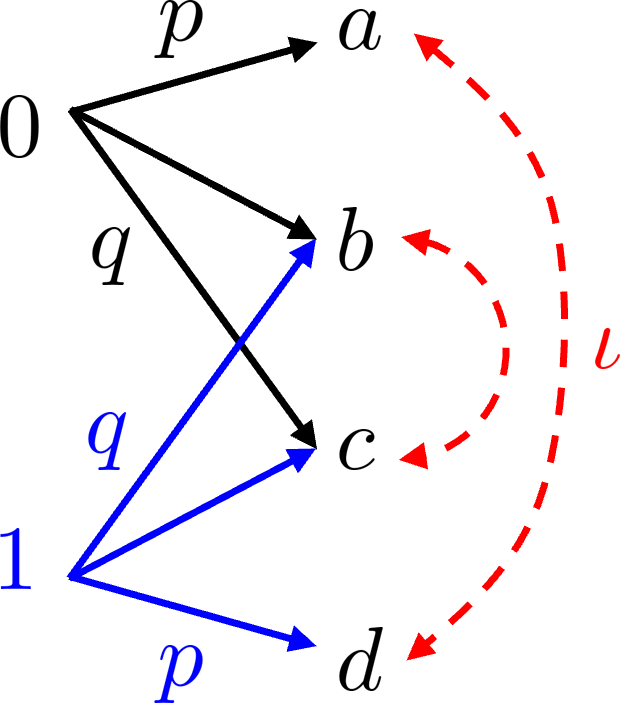
\includegraphics[width=0.2\linewidth]{figures/w3_BMSC.png}
    \caption{Involution of a BMSC.}
\end{figure}
A more general construction of a BMSC channel is shown as follow:
\begin{figure}[H]
    \centering
    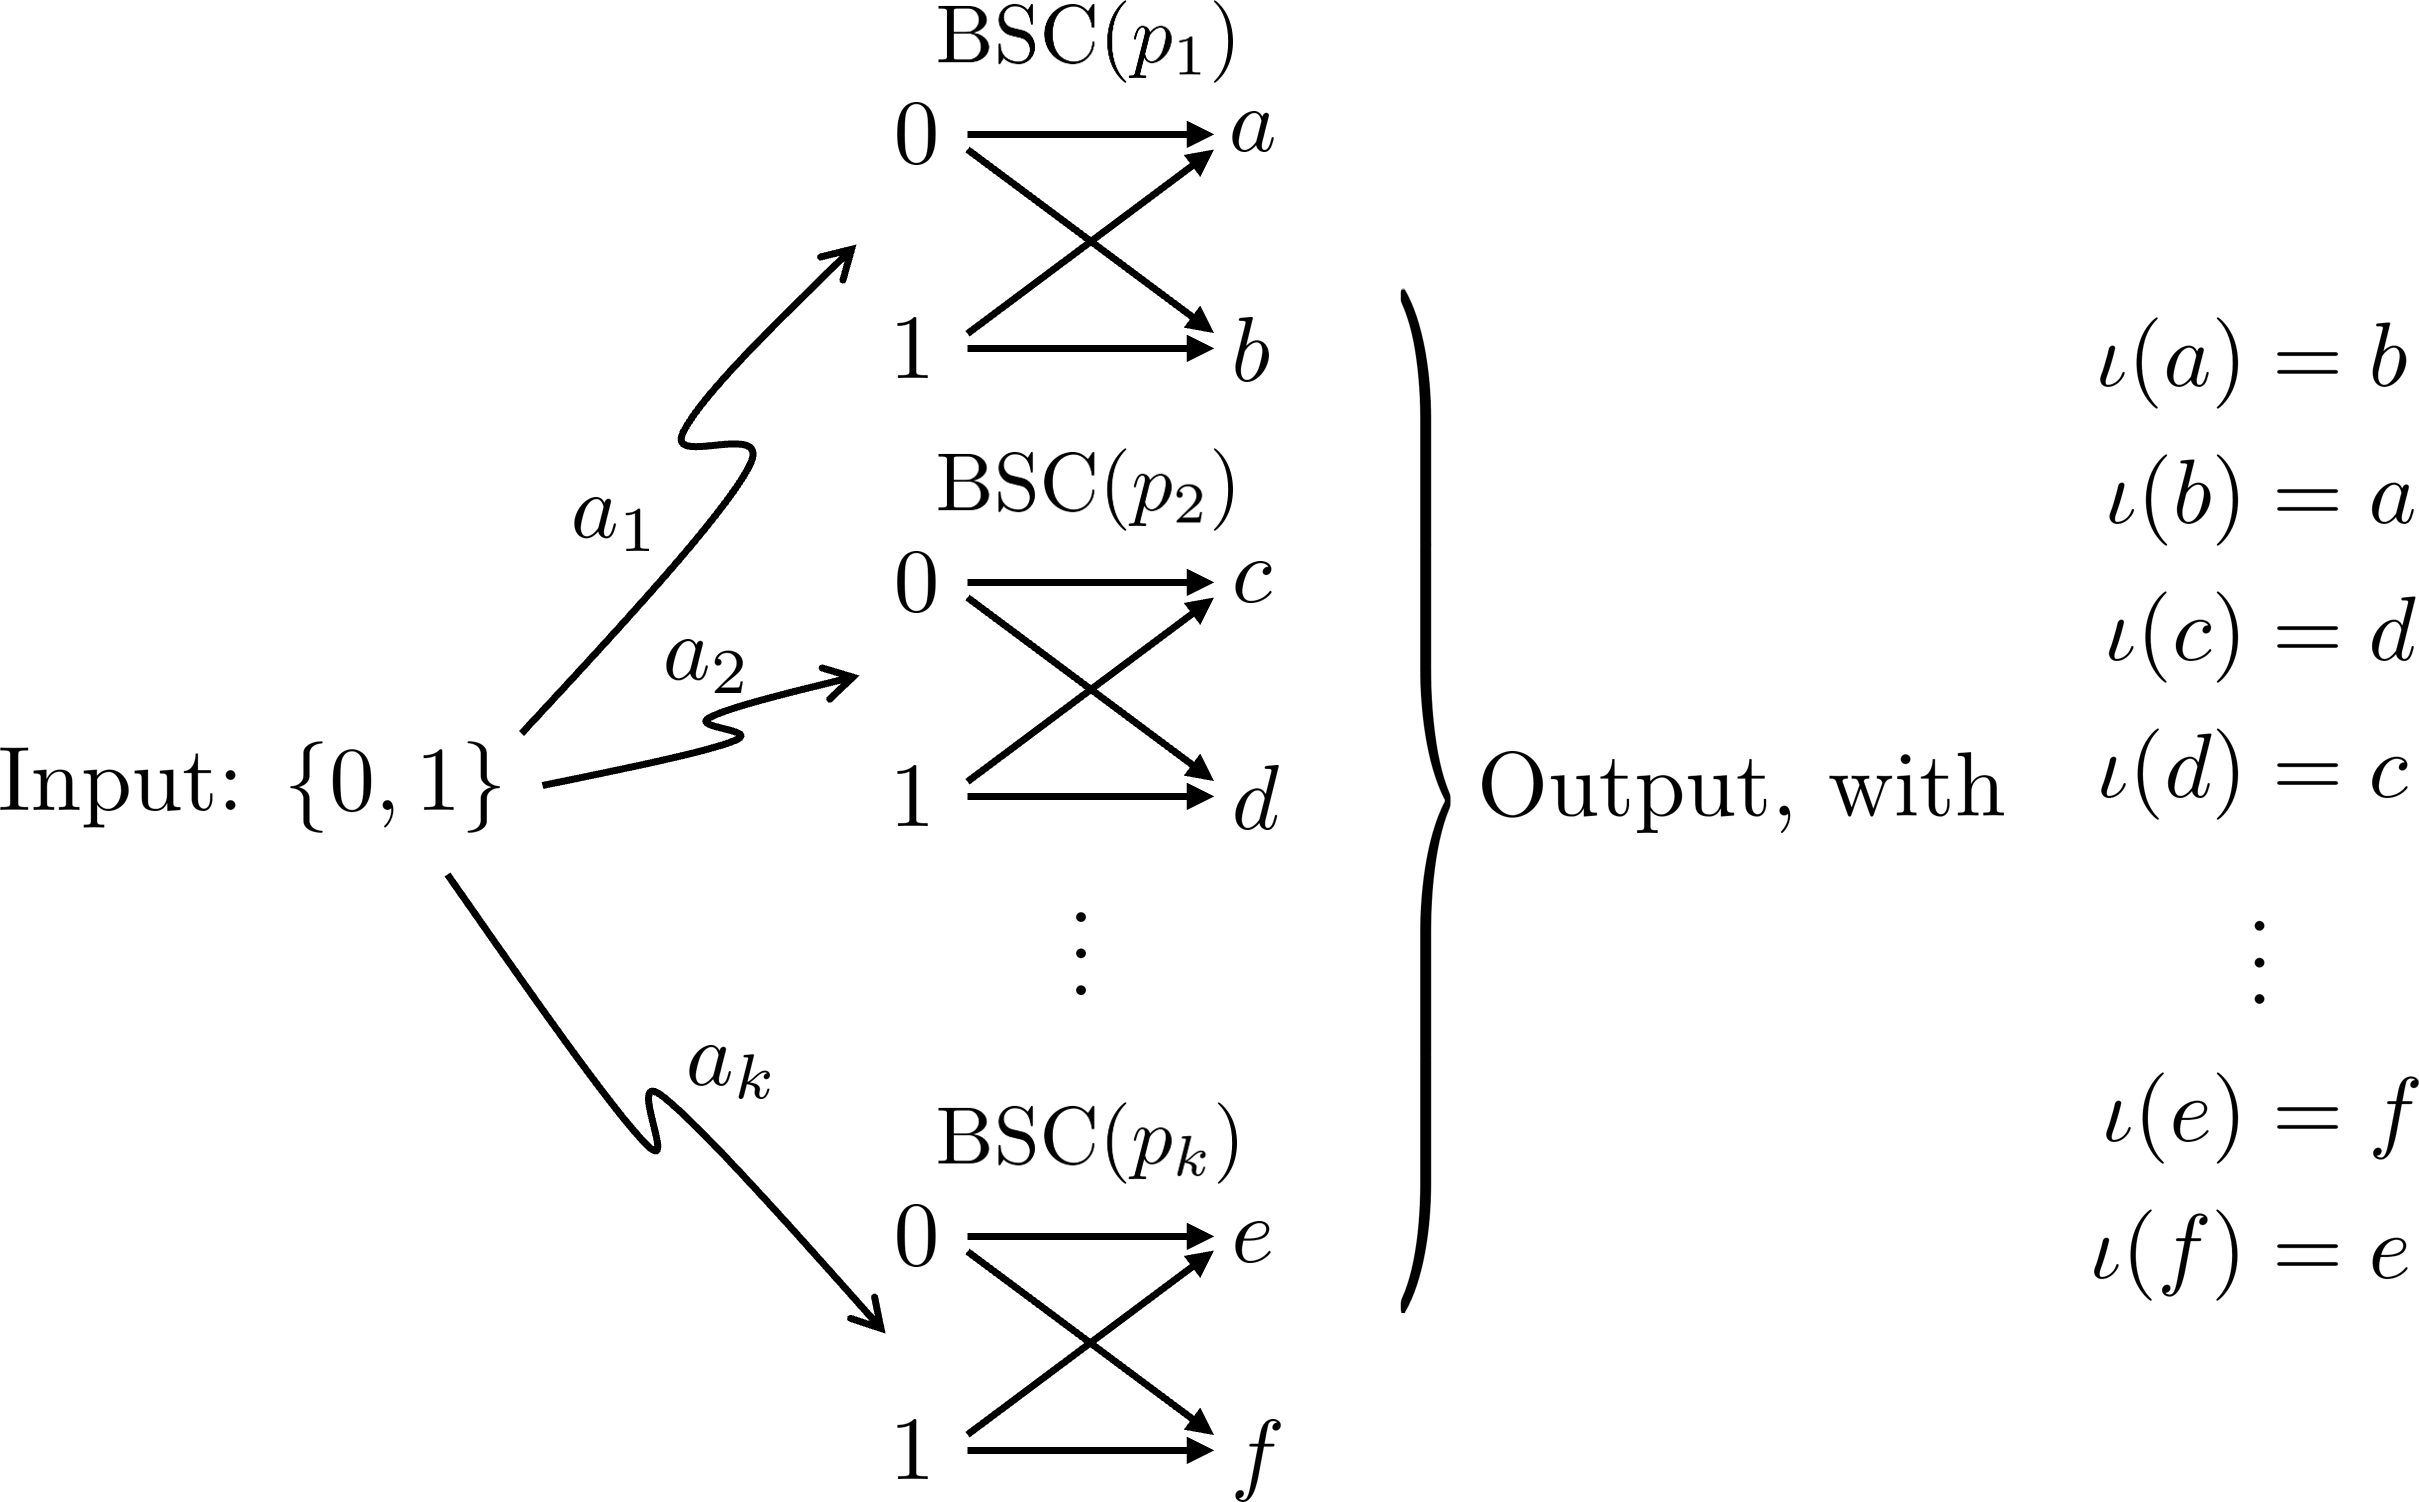
\includegraphics[width=0.7\linewidth]{figures/w3_construct_BMSC.png}
    \caption{Illustration of a general BMSC.}
\end{figure}
By probabilistically assigning a channel $\mathrm{BSC}(p_i)$ with probability $a_i$, we can create seemingly any possible BMSC using BSCs. Note that the involution relations are needed.


In general, we have the following theorem.
\begin{theorem}[BMSC as a Compound of BSCs]
    Given $0<p_1,\ldots,p_k\le\frac{1}{2}$ and $0<a_1,\ldots,a_k<1$ satisfying $a_1+\cdots+a_k=1$, the compound channel
    \begin{equation}
        \sum_{i=1}^k a_i\cdot\mathrm{BSC}(p_i)
    \end{equation}
    is a BMSC. Similarly, any BMSC is equivalent to a decomposition $\sum_{i=1}^k a_i\cdot\mathrm{BSC}(p_i)$.
\end{theorem}
The convex combination of channels corresponds to a probabilistic mixture of the channels.

\begin{remark}
    The decomposition of a BMSC into BSCs holds true even for continuous channels such as an AWGN, where we can replace the summation by an integral:
    \begin{equation*}
        \mathrm{AWGN}(\sigma) = \int A_\sigma(p)\; \mathrm{BSC}(p)\;\dd p.
    \end{equation*}
\end{remark}

For a more general construction and detailed descriptions on BMSC, please refer to the book ``Modern Coding Theory'' \cite{Modern_Coding_Theory} and the paper ``Channel Polarization through the Lens of Blackwell Measures'' \cite{Blackwell_Measure}.


\subsection{The $+$ and $-$ Sub-Channels}
From the above, we know that we can obtain analytical results of any BMSC by analyzing BSCs. In this subsection, we aim to understand the meaning to $\mathrm{BSC}(p)^+$, $\sum a_i\,\mathrm{BSC}(p_i)^+$, $\mathrm{BSC}(p)^-$, and $\sum a_i\,\mathrm{BSC}(p_i)^-$. The paper ``Channel Polarization through the Lens of Blackwell Measures'' \cite{Blackwell_Measure} again provided a detailed and expansive discussion of the following topic.

The most general language that we can use the discussion over the \textit{parallel} and \textit{serial combination} of BSCs, which are denoted by $\mathrm{BSC}(p) \ostar \mathrm{BSC}(q)$ and $\mathrm{BSC}(p) \boxstar \mathrm{BSC}(q)$, respectively. \\

\paragraph{Parallel Combination:}
The parallel combination channel $\mathrm{BSC}(p)\ostar\mathrm{BSC}(q)$ describes what we know about $x\in\{0,1\}$ given the outputs $\mathrm{BSC}(p)(x)$ and $\mathrm{BSC}(q)(x)$. The diagram of the channel is as shown below:
\begin{figure}[H]
    \centering
    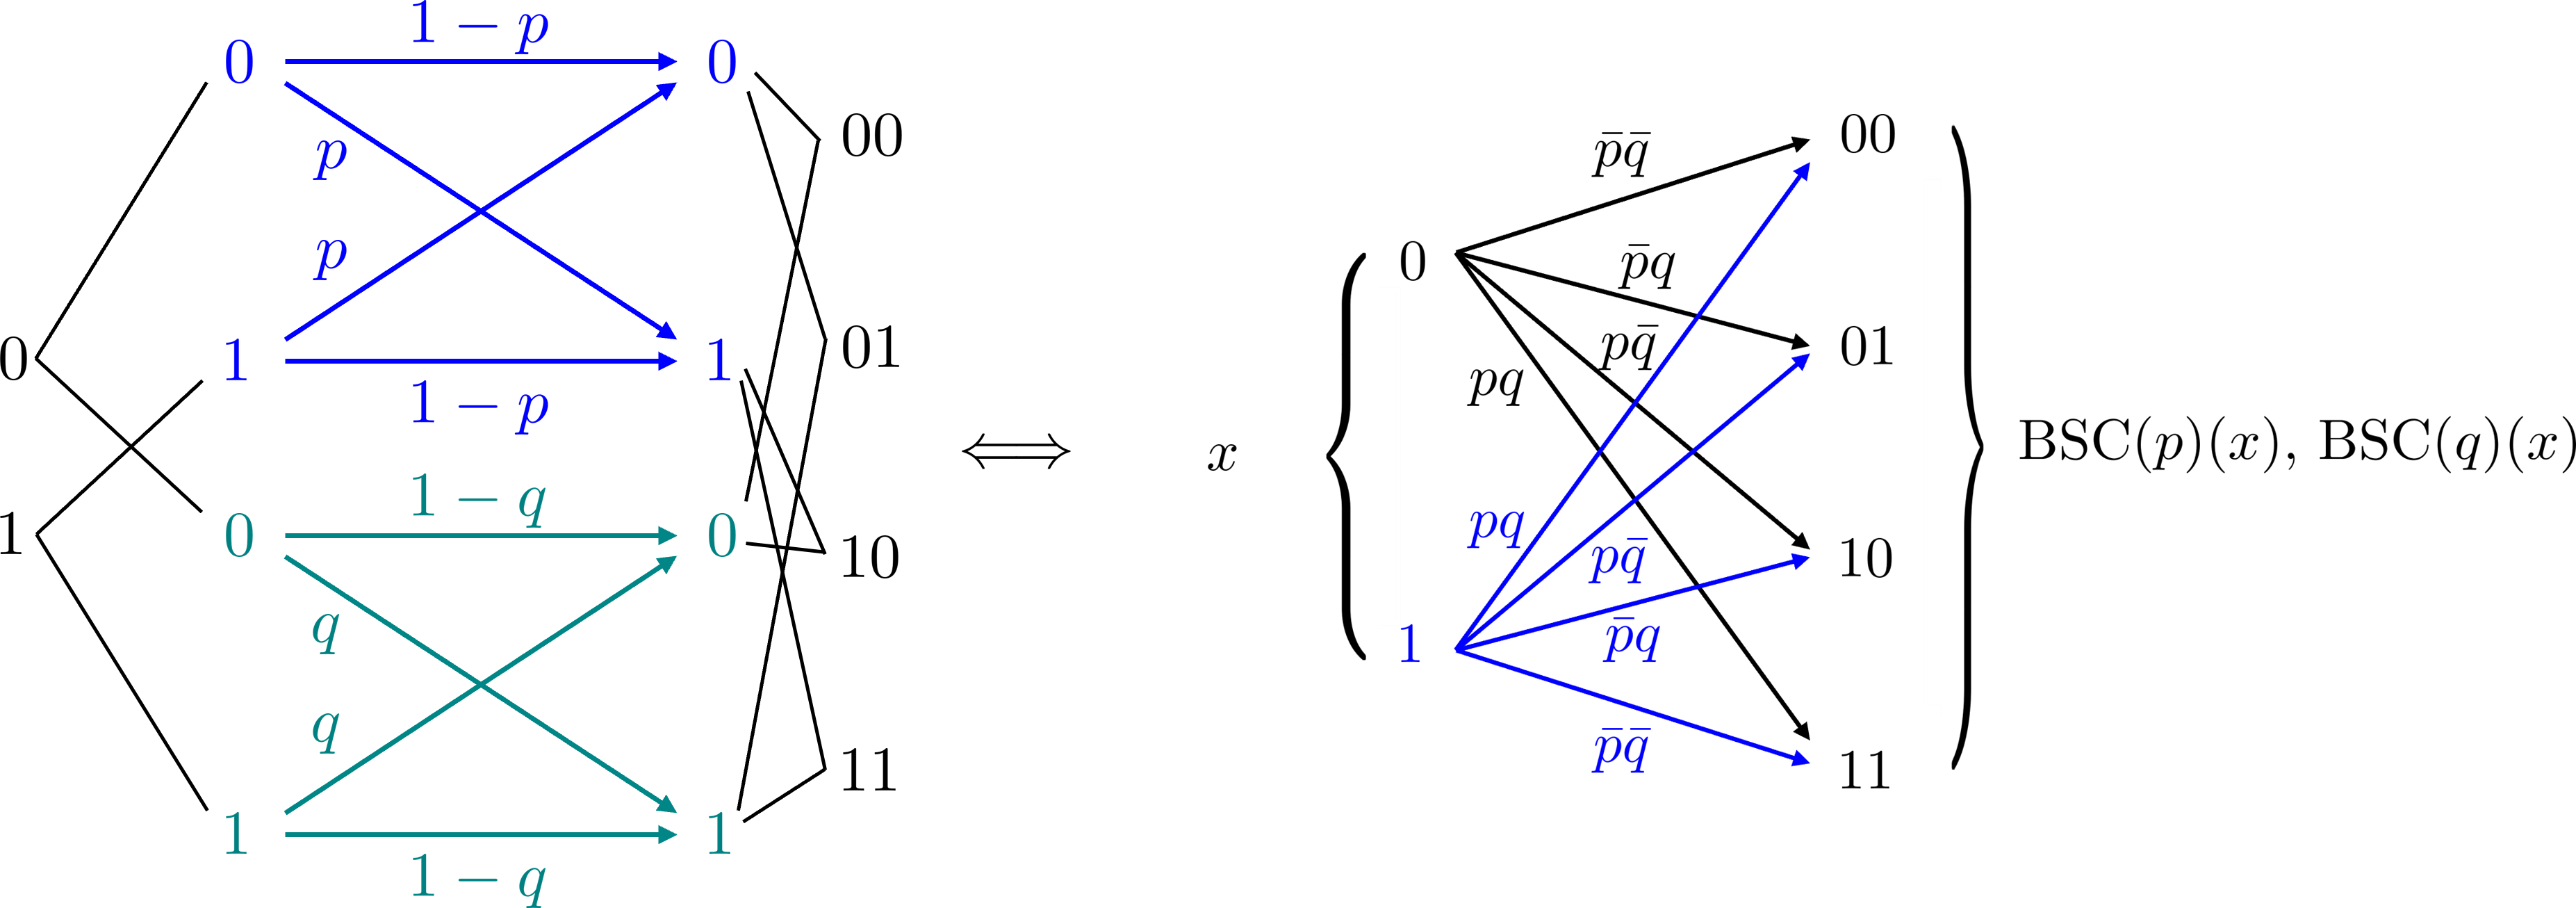
\includegraphics[width=1\linewidth]{figures/w3_parallel_combination.png}
    \caption{Parallel combination of $\textcolor{blue}{\mathrm{BSC}(p)}\ostar\textcolor{teal}{\mathrm{BSC}(q)}$. An input is sent through two parallel channels, with the output compared in parallel to obtain information about the input.}
\end{figure}
By introducing the notation $\bar{x}=1-x$, we have the involution $\iota(x)=\bar{x}$. Furthermore, by an abuse of notation, we also have $\bar{p}=1-p$ and $\bar{q}=1-q$. For an input of $x$, we have the outputs
\begin{align*}
    \begin{cases}
        xx &\text{w.p. }\bar{p}\bar{q},\\
        \bar{x}\bar{x} &\text{w.p. }pq,\\
        x\bar{x} &\text{w.p. }\bar{p}{q},\\
        \bar{x}x &\text{w.p. }{p}\bar{q}.
    \end{cases}
\end{align*}
Henceforth, by considering the involute pairs of $(xx,\bar{x}\bar{x})$ and $(\bar{x}x,x\bar{x})$ as the individual BSC components (since $\iota(xx)=\bar{x}\bar{x}$ and $\iota(\bar{x}x)=x\bar{x}$), we can view the combined channel as
\begin{equation}
    \mathrm{BSC}(p) \ostar \mathrm{BSC}(q) = (pq+\bar{p}\bar{q}) \cdot \mathrm{BSC}\left(\frac{pq}{pq+\bar{p}\bar{q}}\right) + (p\bar{q}+\bar{p}q) \cdot \mathrm{BSC}\left(\frac{p\bar{q}}{p\bar{q}+\bar{p}q}\right).
\end{equation}
The result can be further extended by linearity to
\begin{equation}
    \left(\sum_i a_i \cdot \mathrm{BSC}(p_i)\right) \ostar \left(\sum_i b_i \cdot \mathrm{BSC}(q_i)\right) = \sum_{i,j} a_ib_j \cdot\mathrm{BSC}(p_i)\ostar\mathrm{BSC}(q_j).
\end{equation}


\paragraph{Serial Combination:} The serial combination channel $\mathrm{BSC}(p)\boxstar\mathrm{BSC}(q)$ describes what we know about $x+y$ (mod 2 addition) given the outputs $\mathrm{BSC}(p)(x)$ and $\mathrm{BSC}(q)(y)$. The diagram of the channel is as shown below:
\begin{figure}[H]
    \centering
    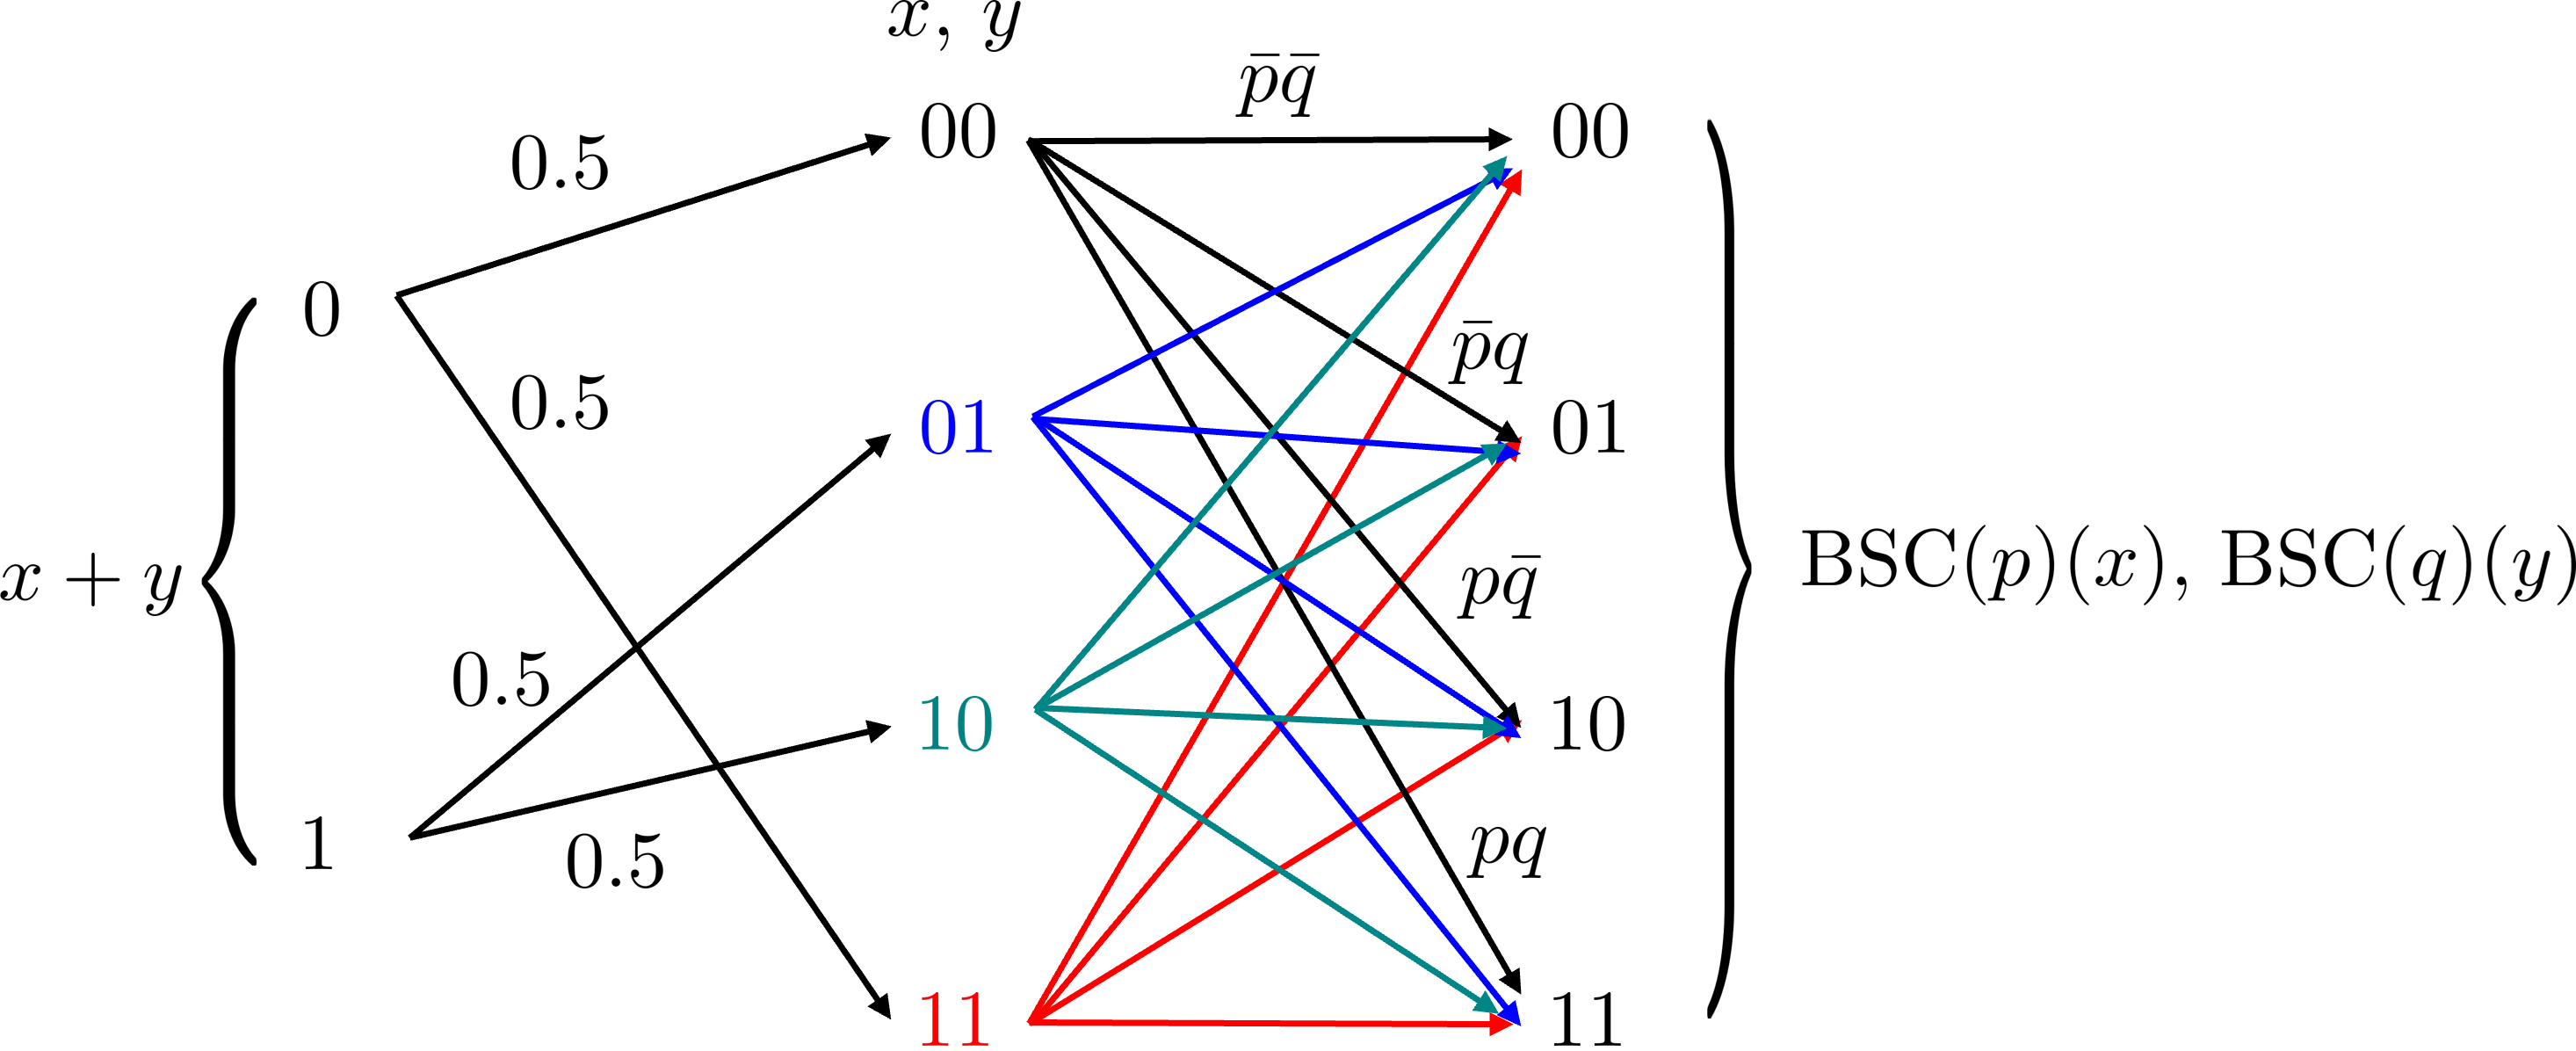
\includegraphics[width=0.8\linewidth]{figures/w3_serial_combination.png}
    \caption{Serial combination of channels. An input is sent through two channels with the output summed together. For the two channels both being BSC, the total effect is equivalent to serial combining the two channels where the output of the first becomes the input of the second.}
    \label{fig:w3_serial}
\end{figure}
The combined channel law is
\begin{align*}
    W(00\vert0) = W(11\vert0) = W(01\vert1) = W(10\vert1) &= \frac{1}{2}(\bar{p}\bar{q}+pq),\\
    W(01\vert0) = W(10\vert0) = W(00\vert1) = W(11\vert1) &= \frac{1}{2}(\bar{p}q+p\bar{q}).
\end{align*}
By considering the super-symbols of involute pairs $A=(00,11)$ and $B=(01,10)$ since the symbols in each super-symbol provides the same information over what $x+y$ is, one can check that the above channel is equivalent to the channel below.
\begin{figure}[H]
    \centering
    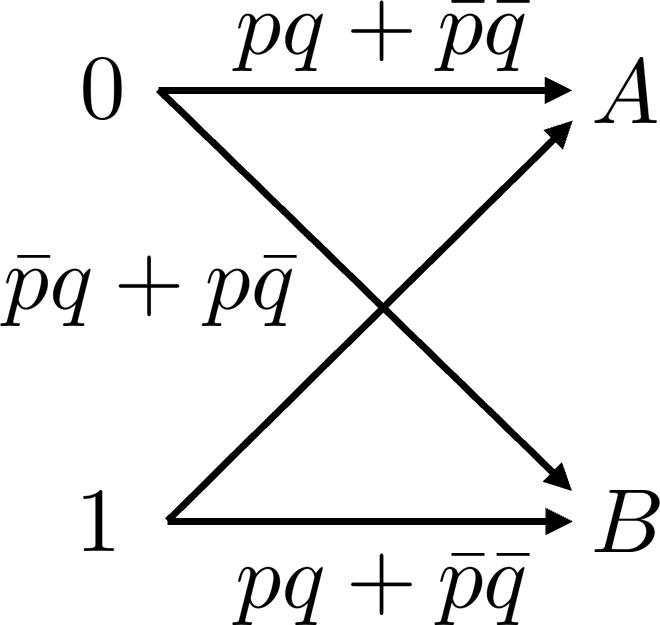
\includegraphics[width=0.2\linewidth]{figures/w3_serial_combination_reduced.png}
    \caption{The serial combination of BSC's is still a BSC.}
\end{figure}
Henceforth, we can view the combined channel as
\begin{equation}
    \mathrm{BSC}(p)\boxstar\mathrm{BSC}(q) = \mathrm{BSC}(pq+\bar{p}\bar{q}).
\end{equation}
The result can be further extended by linearity to
\begin{equation}
    \left(\sum_i a_i \cdot \mathrm{BSC}(p_i)\right) \boxstar \left(\sum_i b_i \cdot \mathrm{BSC}(q_i)\right) = \sum_{i,j} a_ib_j \cdot\mathrm{BSC}(p_i)\boxstar\mathrm{BSC}(q_j).
\end{equation}

\begin{theorem}[Parallel and Serial Combination of BSC]
    For probabilities $p$ and $q$, we have
    \begin{align}
        \mathrm{BSC}(p) \ostar \mathrm{BSC}(q) &= (pq+\bar{p}\bar{q}) \cdot \mathrm{BSC}\left(\frac{pq}{pq+\bar{p}\bar{q}}\right) + (p\bar{q}+\bar{p}q) \cdot \mathrm{BSC}\left(\frac{p\bar{q}}{p\bar{q}+\bar{p}q}\right) \label{w3:BSC_parallel}\\
        \mathrm{BSC}(p)\boxstar\mathrm{BSC}(q) &= \mathrm{BSC}(pq+\bar{p}\bar{q}). \label{w3:BSC_serial}
    \end{align}
\end{theorem}

Note that we can clarify the terms mentioned at the start of this subsection by the following theorem:
\begin{theorem}[The $+$ and $-$ Sub-Channels for BSC]
    For sub-channels of a BSC, we have
    \begin{align}
        \mathrm{BSC}(p)^+ &= \mathrm{BSC}(p)\ostar\mathrm{BSC}(p),\\
        \mathrm{BSC}(p)^- &= \mathrm{BSC}(p)\boxstar\mathrm{BSC}(p).
    \end{align}
\end{theorem}

Lastly, note that for the special case where we are only considering the serial combination of BSCs, and with super-symbols in mind, \autoref{fig:w3_serial} can be transformed into \autoref{fig:w3_serial_BSC}.
\begin{figure}[H]
    \centering
    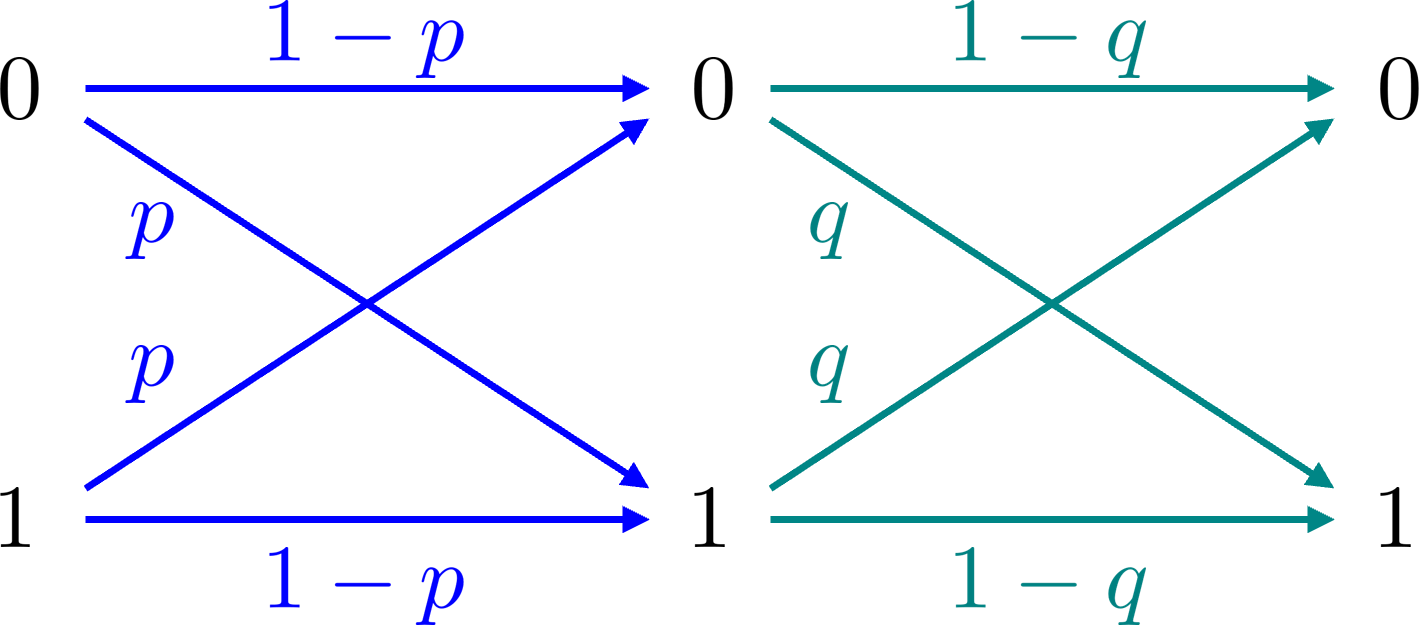
\includegraphics[width=0.5\linewidth]{figures/w3_serial_BSC.png}
    \caption{Serial combination of $\textcolor{blue}{\mathrm{BSC}(p)}\boxstar\textcolor{teal}{BSC}(q)$.}
    \label{fig:w3_serial_BSC}
\end{figure}


By the referenced provided (using the tools derived from the \textit{Blackwell measures}), we have the following general result.
\begin{theorem}[Polar Transform]
    Given two BMSCs $(W_1,\mathcal{Y}_1)$ and $(W_2,\mathcal{Y}_2)$, the \textit{polar transform} maps them into another pair of BMSCs $W_1\ostar W_2$ and $W_1\boxstar W_2$ defined as
    \begin{align}
        (W_1\ostar W_2)(y_1,y_2,u\vert x) &\defeq \frac{1}{2} W_1(y_1\vert x+u) W_2(y_2\vert x), \label{eq:w3_parallel}\\
        (W_1\boxstar W_2)(y_1,y_2\vert x) &\defeq \frac{1}{2} \sum_{u\in\{0,1\}} W_1(y_1\vert x+u) W_2(y_2\vert u) \label{eq:w3_serial}
    \end{align}
    for all $y_1\in\mathcal{Y}_1$, $y_2\in\mathcal{Y}_2$, and $x,u\in\{0,1\}$. The former sub-channel is an improved channel, while the latter is a weaker channel. Especially when $W_1=W_2=W$, we have
    \begin{equation}
        W^+ = W\ostar W \text{ and } W^- = W\boxstar W,
    \end{equation}
    where the equality, if written rigorously, should be an \textit{equivalence} by the \textit{Blackwell measure}.
\end{theorem}
It can be readily seen that under the polar coding scheme: by setting $u_1=u$ and $u_2=x$, with $u$ uniformly distributed, \autoref{eq:w3_parallel} represents the probability of inputting $(u,x)$ and having a channel output of $(y_1,y_2)$ -- if $W_1=W_2=W$, and we group certain symbols into a super-symbol by considering how the polar decoder decodes, this is indeed the channel $W^+$.

Similarly, by setting $u_1=x$ and $u_2=u$, with $u$ uniformly distributed, \autoref{eq:w3_serial} represents the probability of inputting $(x,u)$ and having a channel output of $(y_1,y_2)$ -- if $W_1=W_2=W$, and we group certain symbols into a super-symbol by considering how the polar decoder decodes, this is indeed the channel $W^-$.

% We provide here an alternate proof of this general theorem here, which doesn't require the knowledge of Blackwell measures.
% \begin{proof}
%     Let us consider the two cases separately.
% \begin{enumerate}
%     \item $W_1\ostar W_2$: Under the terminologies of polar code, consider calling $u_1=u$, and $u_2=x$, let us consider the transition probability from $x$ to $(y_1,y_2,u)$ with a uniform prior on $u$. It should be immediate that one arrives at right hand side of \autoref{eq:w3_parallel}. This definition coincide with that of \autoref{eq:w3_parallel_BSC}. For $W_1=W_2$, this is also exactly how we define $W^+$. Hence the equality.

%     \item $W_1\boxstar W_2$: Under the terminologies of polar code, consider calling $u_1=x$, and $u_2=u$, let us consider the transition probability from $x$ to $(y_1,y_2)$ with a uniform prior on $u$. It should be immediate that one arrives at right hand side of \autoref{eq:w3_serial}. This definition coincide with that of \autoref{eq:w3_serial_BSC} in which we consider the transition from $x$ to $y_1+y_2$ if $\mathcal{Y}_1=\mathcal{Y}_2=\{0,1\}$. For $W_1=W_2$, this is also exactly how we define $W^-$. Hence the equality.
% \end{enumerate}
% \end{proof}

Let us demonstrate the theorem above by the following two examples:
\begin{example}
    It can be readily checked that the following equation holds:
    \begin{equation}
        \mathrm{BEC}(x) = \bar{x}\cdot\mathrm{BSC}(1) + x\cdot\mathrm{BSC}(1/2).
    \end{equation}
    Henceforth, we have the two sub-channels calculated to be
    \begin{align*}
        \mathrm{BEC}(x)^+ &= \left(\bar{x} \cdot \mathrm{BSC}(1) + x \cdot \mathrm{BSC}(1/2)\right) \ostar \left(\bar{x} \cdot \mathrm{BSC}(1) + x \cdot \mathrm{BSC}(1/2)\right) \\
        &= \bar{x}^2 \cdot \mathrm{BSC}(1)^+ + x^2 \cdot \mathrm{BSC}(1/2)^+ +2\bar{x}x \cdot \mathrm{BSC}(1)\ostar\mathrm{BSC}(1/2) \\
        &= (1-2x+x^2) \cdot \mathrm{BSC}(1) + x^2 \cdot \mathrm{BSC}(1/2) + (2x-2x^2) \cdot \mathrm{BSC}(1) \\
        &= (1-x^2) \cdot \mathrm{BSC}(1) + x^2 \cdot \mathrm{BSC}(1/2) \\
        &= \mathrm{BEC}(x^2),
    \end{align*}
    \begin{align*}
        \mathrm{BEC}(x)^- &= \left(\bar{x} \cdot \mathrm{BSC}(1) + x \cdot \mathrm{BSC}(1/2)\right) \boxstar \left(\bar{x} \cdot \mathrm{BSC}(1) + x \cdot \mathrm{BSC}(1/2)\right) \\
        &= \bar{x}^2 \cdot \mathrm{BSC}(1)^- + x^2 \cdot \mathrm{BSC}(1/2)^- + 2\bar{x}x \cdot \mathrm{BSC}(1)\boxstar\mathrm{BSC}(1/2) \\
        &= (1-2x+x^2) \cdot \mathrm{BSC}(1) + x^2 \cdot \mathrm{BSC}(1/2) + (2x-2x^2) \cdot \mathrm{BSC}(1/2) \\
        &= (1-2x+x^2) \cdot \mathrm{BSC}(1) + (2x-x^2) \cdot \mathrm{BSC}(1/2)\\
        &= \mathrm{BEC}(2x-x^2).
    \end{align*}
    Thus, we have proven the sub-channel laws of polar code on BEC observed in the first chapter, where $\ostar$ results in a better sub-channel, and $\boxstar$ results in a worse sub-channel.
\end{example}
\begin{example}
    The sub-channels to BEC can also be directly calculated from the polar transformation. Note that $W_1=W_2 = \mathrm{BEC}(x)$ and $\mathcal{Y}_1=\mathcal{Y}_2=\{0,1,\mathcal{E}\}$. Hence, by abbreviating $W\ostar W$ as $W_p$, we have for parallel combination
    \begin{align*}
        \frac{1}{2}\bar{x}^2 &= W_p(0,0,0\vert0) = W_p(1,1,0\vert1) = W_p(1,0,1\vert0) = W_p(0,1,1\vert1), \\
        \frac{1}{2}\bar{x}x &= W_p(\mathcal{E},0,0\vert0) = W_p(\mathcal{E},1,0\vert1) = W_p(\mathcal{E},0,1\vert0) = W_p(\mathcal{E},1,1\vert1) \\
        &= W_p(0,\mathcal{E},0\vert0) = W_p(1,\mathcal{E},0\vert1) = W_p(1,\mathcal{E},1\vert0) = W_p(0,\mathcal{E},1\vert1), \\
        \frac{1}{2}x^2 &= W_p(\mathcal{E},\mathcal{E},0\vert0) = W_p(\mathcal{E},\mathcal{E},0\vert1) = W_p(\mathcal{E},\mathcal{E},1\vert0) = W_p(\mathcal{E},\mathcal{E},1\vert1),
    \end{align*}
    all the other cases have a value of 0. Consider the following disjoint sets of possible outputs,
    \begin{align*}
        \mathcal{S}_0 &= \{(0,0,0),(1,0,1),(\mathcal{E},0,0),(0,\mathcal{E},0),(\mathcal{E},0,1),(1,\mathcal{E},1)\}, \\
        \mathcal{S}_1 &= \{(1,1,0),(0,1,1),(\mathcal{E},1,0),(1,\mathcal{E},0),(\mathcal{E},1,1),(0,\mathcal{E},1)\}, \\
        \mathcal{S}_\mathcal{E} &= \{(\mathcal{E},\mathcal{E},0),(\mathcal{E},\mathcal{E},1)\},
    \end{align*}
    they can be viewed as super-symbols, where the polar decoder will decode $\mathcal{S}_y$ into $y$. Then we can calculate the probability of each set happening:
    \begin{align*}
        1-x^2 &= \mathrm{Pr}\{\mathcal{S}_0\vert0\} = \mathrm{Pr}\{\mathcal{S}_1\vert1\},\\
        0 &= \mathrm{Pr}\{\mathcal{S}_1\vert0\} = \mathrm{Pr}\{\mathcal{S}_0\vert1\},\\
        x^2 &= \mathrm{Pr}\{\mathcal{S}_\mathcal{E}\vert0\} = \mathrm{Pr}\{\mathcal{S}_\mathcal{E}\vert1\}.
    \end{align*}
    Hence, we have that $\mathrm{BEC}(x)^+ = \mathrm{BEC}(x)\ostar\mathrm{BEC}(x) \equiv \mathrm{BEC}(x^2)$.

    Next, let us analyze the serial combination. By abbreviating $W\boxstar W$ as $W_s$, we have
    \begin{align*}
        \frac{1}{2}\bar{x}^2 &= W_s(0,0\vert0) = W_s(1,1\vert0) = W_s(0,1\vert1) = W_s(1,0\vert1), \\
        \frac{1}{2}\bar{x}x &= W_s(\mathcal{E},0\vert0) = W_s(\mathcal{E},1\vert0) = W_s(\mathcal{E},1\vert1) = W_s(\mathcal{E},0\vert1) \\
        &= W_s(0,\mathcal{E}\vert0) = W_s(1,\mathcal{E}\vert0) = W_s(0,\mathcal{E}\vert1) = W_s(1,\mathcal{E}\vert1), \\
        x^2 &= W_s(\mathcal{E},\mathcal{E}\vert0) = W_s(\mathcal{E},\mathcal{E}\vert1).
    \end{align*}
    all the other cases have a value of 0. Consider the following disjoint sets of possible outputs,
    \begin{align*}
        \mathcal{S}_0 &= \{(0,0),(1,1)\}, \\
        \mathcal{S}_1 &= \{(0,1),(1,0)\}, \\
        \mathcal{S}_\mathcal{E} &= \{(\mathcal{E},0),(\mathcal{E},1),(0,\mathcal{E}),(1,\mathcal{E}),(\mathcal{E},\mathcal{E})\},
    \end{align*}
    they are again viewed as super-symbols, representing the decoding scheme. Then we can calculate the probability of each set happening:
    \begin{align*}
        \bar{x}^2 &= \mathrm{Pr}\{\mathcal{S}_0\vert0\} = \mathrm{Pr}\{\mathcal{S}_1\vert1\},\\
        0 &= \mathrm{Pr}\{\mathcal{S}_1\vert0\} = \mathrm{Pr}\{\mathcal{S}_0\vert1\},\\
        2x-x^2 &= \mathrm{Pr}\{\mathcal{S}_\mathcal{E}\vert0\} = \mathrm{Pr}\{\mathcal{S}_\mathcal{E}\vert1\}.
    \end{align*}
    Hence, we have that $\mathrm{BEC}(x)^- = \mathrm{BEC}(x)\boxstar\mathrm{BEC}(x) \equiv \mathrm{BEC}(2x-x^2)$.
\end{example}

By the tedious work above, we have successfully proven the two roads to be equivalent. It should be noted that the grouping of the super-symbols are achieved by considering the polar decoder, which is a decoding scheme based on maximum likelihood test.

\begin{remark}
    Channels can have arbitrary output alphabets, and need not be integers that can be added. For both serial and parallel combinations, we talked about \textit{aggregating} the output symbols in certain ways (for example, adding the symbols as accounting for parity or creating super-symbols), but these interpretations are actually based on the fact that we treat \textit{symbols posing the same coding challenge as the same}.

    We cal a BMSC channel $W:\{0,1\}\rightarrow\mathcal{Y}_W$ a \textit{symbol aggregation} of another BMSC $V:\{0,1\}\rightarrow\mathcal{Y}_V$ if there exists a map $\pi:\mathcal{Y}_V\rightarrow\mathcal{Y}_W$ satisfying
    \begin{equation}\begin{aligned}
        V(y\mid0):V(y\mid1) &= W(\pi(y)\mid0):W(\pi(y)\mid1), \\
        \sum_{v\in\pi^{-1}(y)}V(v\mid0)+V(v\mid1) &= W(y\mid0):W(y\mid1).
    \end{aligned}\end{equation}
\end{remark}
